\documentclass[a4paper,11pt]{book}
%\documentclass[a4paper,twoside,11pt,titlepage]{book}
\usepackage{listings}
\usepackage[utf8]{inputenc}
\usepackage[spanish]{babel}
\usepackage{amsthm}
\usepackage{amsfonts}
\usepackage{amsmath}


%\setbeamercovered{transparent}
%\usepackage{minted}
%%\usepackage{scrhack}
\usepackage{listings}

\usepackage[T1]{fontenc}
\usepackage{verbatim}

\usepackage{multicol}
\usepackage{graphicx}

\usepackage[backend=bibtex, style=numeric]{biblatex}
\addbibresource{bibliografia.bib}


\newtheorem{teorema}{Teorema}
\newtheorem{lema}[teorema]{Lema}
\newtheorem{definicion}[teorema]{Definición}
\newtheorem{proposicion}[teorema]{Proposición}
\newtheorem{corolario}[teorema]{Corolario}
\newtheorem{ejemplo}{Ejemplo}
\newtheorem{observacion}{Observación}

% \usepackage[style=list, number=none]{glossary} %
%\usepackage{titlesec}
%\usepackage{pailatino}

\decimalpoint
\usepackage{dcolumn}
\newcolumntype{.}{D{.}{\esperiod}{-1}}
\makeatletter
\addto\shorthandsspanish{\let\esperiod\es@period@code}
\makeatother


%\usepackage[chapter]{algorithm}
\RequirePackage{verbatim}
%\RequirePackage[Glenn]{fncychap}
\usepackage{fancyhdr}
\usepackage{graphicx}
\usepackage{afterpage}

\usepackage{longtable}

\usepackage[pdfborder={000}]{hyperref} %referencia

% ********************************************************************
% Re-usable information
% ********************************************************************
\newcommand{\myTitle}{Título del proyecto\xspace}
\newcommand{\myDegree}{Grado en ...\xspace}
\newcommand{\myName}{Nombre Apllido1 Apellido2 (alumno)\xspace}
\newcommand{\myProf}{Nombre Apllido1 Apellido2 (tutor1)\xspace}
\newcommand{\myOtherProf}{Nombre Apllido1 Apellido2 (tutor2)\xspace}
%\newcommand{\mySupervisor}{Put name here\xspace}
\newcommand{\myFaculty}{Escuela Técnica Superior de Ingenierías Informática y de
Telecomunicación\xspace}
\newcommand{\myFacultyShort}{E.T.S. de Ingenierías Informática y de
Telecomunicación\xspace}
\newcommand{\myDepartment}{Departamento de ...\xspace}
\newcommand{\myUni}{\protect{Universidad de Granada}\xspace}
\newcommand{\myLocation}{Granada\xspace}
\newcommand{\myTime}{\today\xspace}
\newcommand{\myVersion}{Version 0.1\xspace}


\hypersetup{
pdfauthor = {\myName (email (en) ugr (punto) es)},
pdftitle = {\myTitle},
pdfsubject = {},
pdfkeywords = {palabra_clave1, palabra_clave2, palabra_clave3, ...},
pdfcreator = {LaTeX con el paquete ....},
pdfproducer = {pdflatex}
}

%\hyphenation{}


%\usepackage{doxygen/doxygen}
%\usepackage{pdfpages}
\usepackage{url}
\usepackage{colortbl,longtable}
\usepackage[stable]{footmisc}
%\usepackage{index}

%\makeindex
%\usepackage[style=long, cols=2,border=plain,toc=true,number=none]{glossary}
% \makeglossary

% Definición de comandos que me son tiles:
%\renewcommand{\indexname}{Índice alfabético}
%\renewcommand{\glossaryname}{Glosario}

\pagestyle{fancy}
\fancyhf{}
\fancyhead[LO]{\leftmark}
\fancyhead[RE]{\rightmark}
\fancyhead[RO,LE]{\textbf{\thepage}}
\renewcommand{\chaptermark}[1]{\markboth{\textbf{#1}}{}}
\renewcommand{\sectionmark}[1]{\markright{\textbf{\thesection. #1}}}

\setlength{\headheight}{1.5\headheight}

\newcommand{\HRule}{\rule{\linewidth}{0.5mm}}
%Definimos los tipos teorema, ejemplo y definición podremos usar estos tipos
%simplemente poniendo \begin{teorema} \end{teorema} ...




%%%%%\newtheorem{teorema}{Teorema}[chapter]
%%%%%\newtheorem{ejemplo}{Ejemplo}[chapter]
%%%%%\newtheorem{definicion}{Definición}[chapter]


\definecolor{gray97}{gray}{.97}
\definecolor{gray75}{gray}{.75}
\definecolor{gray45}{gray}{.45}
\definecolor{gray30}{gray}{.94}
 
\lstset{ frame=Ltb,
     framerule=0.5pt,
     aboveskip=0.5cm,
     framextopmargin=3pt,
     framexbottommargin=3pt,
     framexleftmargin=0.1cm,
     framesep=0pt,
     rulesep=.4pt,
     backgroundcolor=\color{gray97},
     rulesepcolor=\color{black},
     %
     stringstyle=\ttfamily,
     showstringspaces = false,
     basicstyle=\scriptsize\ttfamily,
     commentstyle=\color{gray45},
     keywordstyle=\bfseries,
     %
     numbers=left,
     numbersep=6pt,
     numberstyle=\tiny,
     numberfirstline = false,
     breaklines=true,
   }

% minimizar fragmentado de listados
\lstnewenvironment{listing}[1][]
   {\lstset{#1}\pagebreak[0]}{\pagebreak[0]}

\lstdefinestyle{CodigoC}
   {
	basicstyle=\scriptsize,
	frame=single,
	language=C,
	numbers=left
   }
\lstdefinestyle{CodigoC++}
   {
	basicstyle=\small,
	frame=single,
	backgroundcolor=\color{gray30},
	language=C++,
	numbers=left
   }

 
\lstdefinestyle{Consola}
   {basicstyle=\scriptsize\bf\ttfamily,
    backgroundcolor=\color{gray30},
    frame=single,
    numbers=none
   }


\newcommand{\bigrule}{\titlerule[0.5mm]}


%Para conseguir que en las páginas en blanco no ponga cabecerass
\makeatletter
\def\clearpage{%
  \ifvmode
    \ifnum \@dbltopnum =\m@ne
      \ifdim \pagetotal <\topskip
        \hbox{}
      \fi
    \fi
  \fi
  \newpage
  \thispagestyle{empty}
  \write\m@ne{}
  \vbox{}
  \penalty -\@Mi
}
\makeatother


\usepackage{pdfpages}
\begin{document}
\begin{titlepage}
 
 
\newlength{\centeroffset}
\setlength{\centeroffset}{-0.5\oddsidemargin}
\addtolength{\centeroffset}{0.5\evensidemargin}
\thispagestyle{empty}

\noindent\hspace*{\centeroffset}\begin{minipage}{\textwidth}

\centering

\includegraphics[width=0.3\textwidth]{imagenes/logougr_new.png}\\[1.4cm]

\textsc{ \Large TRABAJO FIN DE GRADO\\[0.2cm]}
\textsc{ EN INGENIERÍA INFORMÁTICA Y MATEMÁTICAS }\\[1cm]

% Upper part of the page
% 
% Title
{\Huge\bfseries Rigidez de ovaloides : Teorema de Cohn-Vossen. Visualización computacional\\
}
%%%%\noindent\rule[-1ex]{\textwidth}{3pt}\\[3.5ex]
%%%%{\large\bfseries Subtitulo del Proyecto}
\end{minipage}

\vspace{2.5cm}
\noindent\hspace*{\centeroffset}\begin{minipage}{\textwidth}
\centering

\textbf{Autor}\\ {Eva María González García}\\[2.5ex]
${ }$\\
\textbf{Directores}\\
%%{
\begin{multicols}{2}
		Francisco Urbano Pérez-Aranda\\
		\columnbreak
Carlos Ureña Almagro
\end{multicols}%%}\\[2cm]

${ }$\\
\begin{multicols}{2}%%7}
%%	
%%	\hfill\columnbreak
%%	
%%	\hfill\columnbreak
%%	
%%	\hfill\columnbreak
%%	
  %% \hfill\columnbreak
           
%%\hfill\columnbreak

\hfill
\includegraphics[width=0.09\textwidth]{imagenes/orbitasPeq.png}\\[0.1cm]
\columnbreak
%%\hfill
\raggedright
\includegraphics[width=0.09\textwidth]{imagenes/logo_etsiit.png}\\[0.1cm]
\end{multicols}
\textsc{Facultad de Ciencias}\\
\textsc{y}\\
\textsc{E. T. S. de Ingenierías Informática y de Telecomunicación}\\
%%%%%%%
\includegraphics[width=0.3\textwidth]{imagenes/etsiit_logo.png}\\[0.1cm]
%%%%%%%\textsc{Escuela Técnica Superior de Ingenierías Informática y de Telecomunicación}\\
%%%%%%\textsc{---}\\
%%%%%%Granada, mes de 201
\end{minipage}
%\addtolength{\textwidth}{\centeroffset}
%\vspace{\stretch{2}}
\end{titlepage}



\chapter*{}
%\thispagestyle{empty}
%\cleardoublepage

%\thispagestyle{empty}

\begin{titlepage}
 
 
\setlength{\centeroffset}{-0.5\oddsidemargin}
\addtolength{\centeroffset}{0.5\evensidemargin}
\thispagestyle{empty}

\noindent\hspace*{\centeroffset}\begin{minipage}{\textwidth}

\centering
%
\includegraphics[width=0.9\textwidth]{imagenes/logo_ugr.jpg}\\[1.4cm]

%\textsc{ \Large PROYECTO FIN DE CARRERA\\[0.2cm]}
%\textsc{ INGENIERÍA EN INFORMÁTICA}\\[1cm]
% Upper part of the page
% 

 \vspace{3.3cm}

%si el proyecto tiene logo poner aquí

\includegraphics[width=0.3\textwidth]{imagenes/logougr_new.png}\\[1.4cm]

 \vspace{0.5cm}

% Title

{\Huge\bfseries Rigidez de ovaloides : Teorema de Cohn-Vossen. Visualización computacional\\
}
%%%%\noindent\rule[-1ex]{\textwidth}{3pt}\\[3.5ex]
%%%%{\large\bfseries Subtítulo del proyecto.\\[4cm]}
\end{minipage}

\vspace{2.5cm}
\noindent\hspace*{\centeroffset}\begin{minipage}{\textwidth}
\centering

\textbf{Autor}\\ {Eva María González García}\\[2.5ex]
\textbf{Directores}\\
{Francisco Urbano Pérez-Aranda\\
Carlos Ureña Almagro}\\[2cm]
%
\includegraphics[width=0.15\textwidth]{imagenes/tstc.png}\\[0.1cm]
%\textsc{Departamento de Teoría de la Señal, Telemática y Comunicaciones}\\
%\textsc{---}\\
%Granada, mes de 201
\end{minipage}
%\addtolength{\textwidth}{\centeroffset}
\vspace{\stretch{2}}

 
\end{titlepage}






\cleardoublepage
\thispagestyle{empty}

\begin{center}
{\large\bfseries Título del Proyecto: Subtítulo del proyecto}\\
\end{center}
\begin{center}
Nombre Apellido1 Apellido2 (alumno)\\
\end{center}

%\vspace{0.7cm}
\noindent{\textbf{Palabras clave}: palabra\_clave1, palabra\_clave2, palabra\_clave3, ......}\\

\vspace{0.7cm}
\noindent{\textbf{Resumen}}\\

Poner aquí el resumen.
\cleardoublepage


\thispagestyle{empty}


\begin{center}
{\large\bfseries Project Title: Project Subtitle}\\
\end{center}
\begin{center}
First name, Family name (student)\\
\end{center}

%\vspace{0.7cm}
\noindent{\textbf{Keywords}: Keyword1, Keyword2, Keyword3, ....}\\

\vspace{0.7cm}
\noindent{\textbf{Abstract}}\\

Write here the abstract in English.

\chapter*{}
\thispagestyle{empty}

\noindent\rule[-1ex]{\textwidth}{2pt}\\[4.5ex]

Yo, \textbf{Nombre Apellido1 Apellido2}, alumno de la titulación TITULACIÓN de la \textbf{Escuela Técnica Superior
de Ingenierías Informática y de Telecomunicación de la Universidad de Granada}, con DNI XXXXXXXXX, autorizo la
ubicación de la siguiente copia de mi Trabajo Fin de Grado en la biblioteca del centro para que pueda ser
consultada por las personas que lo deseen.

\vspace{6cm}

\noindent Fdo: Nombre Apellido1 Apellido2

\vspace{2cm}

\begin{flushright}
Granada a X de mes de 201 .
\end{flushright}


\chapter*{}
\thispagestyle{empty}

\noindent\rule[-1ex]{\textwidth}{2pt}\\[4.5ex]

D. \textbf{Nombre Apellido1 Apellido2 (tutor1)}, Profesor del Área de XXXX del Departamento YYYY de la Universidad de Granada.

\vspace{0.5cm}

D. \textbf{Nombre Apellido1 Apellido2 (tutor2)}, Profesor del Área de XXXX del Departamento YYYY de la Universidad de Granada.


\vspace{0.5cm}

\textbf{Informan:}

\vspace{0.5cm}

Que el presente trabajo, titulado \textit{\textbf{Título del proyecto, Subtítulo del proyecto}},
ha sido realizado bajo su supervisión por \textbf{Nombre Apellido1 Apellido2 (alumno)}, y autorizamos la defensa de dicho trabajo ante el tribunal
que corresponda.

\vspace{0.5cm}

Y para que conste, expiden y firman el presente informe en Granada a X de mes de 201 .

\vspace{1cm}

\textbf{Los directores:}

\vspace{5cm}

\noindent \textbf{Nombre Apellido1 Apellido2 (tutor1) \ \ \ \ \ Nombre Apellido1 Apellido2 (tutor2)}

%\chapter*{Agradecimientos}
%\thispagestyle{empty}

%       \vspace{1cm}


%Poner aquí agradecimientos...




%\frontmatter
%\tableofcontents
%\listoffigures
%\listoftables
%
%\mainmatter
%\setlength{\parskip}{5pt}
%
%

\tableofcontents




\chapter*{Introducción}


${ }$\\
$\textbf{RIGIDEZ, OVALOIDES Y OTROS RESULTADOS Y CONCEPTOS}$
${ }$\\

Para llegar al resultado principal que se pretende demostrar primero vamos a ver algunos resultados y definiciones que son necesarios para comprender un poco mejor lo que se quiere mostrar. Algunos de estos resultados no estarán demostrados debido a su extensión o complejidad y a que se alejan del propósito de este trabajo.
${ }$\\

En esta primera parte del trabajo vamos a ver que superficies sabemos que son rígidas, como ya veremos estas son las esferas y mas generalmente los ovaloides. Para ello es importante tener en cuenta algunos conceptos y resultados. Como son los siguientes.

\begin{definicion}\label{def:isom} % label para cuando haga una referencia.
	Dadas dos superficies S y $S'$ y dada una aplicación $f : S \longrightarrow S'$, diremos que $f$ es una \underline{\textbf{isometría}} si es un difeomorfismo y además conserva la primera forma fundamental, esto es, $\langle df_p(u), df_p(v)\rangle = \langle u, v\rangle$ $\forall p \in S$ y $\forall u,v \in T_p S$.
\end{definicion}

Dicho esto, dos superficies son isométricas si existe una isometría que nos lleva una superficie en la otra.

\begin{definicion}
	Llamaremos \underline{\textbf{movimiento rígido}} de $\mathbb{R}^3$ a las aplicaciones de la forma $f(x) = Ax + b$ donde A en una matriz ortogonal de orden 3 y $b \in \mathbb{R}^3$, es decir $A \in O(3)$ con lo cual cumple que $AA^{t} = I_{n}$.
\end{definicion}

\begin{definicion}
	Llamaremos \underline{\textbf{ovaloide}} a una superficie $S \in \mathbb{R}^3$ compacta y conexa cuya curvatura de Gauss sea siempre positiva.
	
	También, si $S$ es un ovaloide, $N =$ normal interior de $S$ y $\sigma =$ segunda forma fundamental respecto a $N$. Entonces, $\sigma > 0$.
\end{definicion}

\begin{definicion}
	Diremos que $S \subset \mathbb{R}^3$ es una \underline{\textbf{superficie rígida}} cuando toda isometría $f : S \to S'$ sea la restrición de un movimiento rígido.
\end{definicion}

Mas intuitivamente, los movimientos rígidos son funciones que cumplen $\langle f(u), f(v) \rangle = \langle u, v \rangle$, es decir, que la distancia entre puntos, siendo la distancia la longitud de la linea recta que los une, se conserva al aplicar $f$.

También tenemos que las isometrías son aplicaciones que conservan la distancia entre puntos de la superficie, tomando la distancia entre dos puntos la longitud de la geodésica que une cada punto. Esto quiere decir que si tomamos dos puntos cualquiera de $S$ la distancia de los puntos imagen sigue siendo la misma. Vamos a ver que esto es cierto con la siguiente proposición:

\begin{proposicion}
	$f : S \to S'$ es una isometría, si y sólo si, $f$ conserva la longitud de las curvas.
\end{proposicion}

\begin{proof}
	${}$\\
	
	Si tomamos $\alpha : [a,b] \to S$ una curva diferenciable en la superficie $S$, entonces la longitud de la curva imagen es la siguiente
	\[
	L^{b}_{a} (f \circ \alpha) = \int^{b}_{a} |(f \circ \alpha)'(t)| dt = \int^{b}_{a} |(df)_{\alpha(t)}(\alpha'(t)))|.
	\]
	como $f$ es isometría, tenemos
	\[
	L^{b}_{a} (f \circ \alpha) = \int^{b}_{a} |\alpha'(t)| = L^{a}_{b} (\alpha).
	\]
	
	Ahora veamos el recíproco, tomando $p \in S$ y $v \in T_p S$, existe una curva diferenciable $\alpha : (-\epsilon, \epsilon) \to S$ para cierto $\epsilon > 0$ tal que $\alpha(0) = p$ y $\alpha'(0) = v$. Como $f$ conserva las distancias, tenemos
	\[
	\int^{t}_{0}|(f \circ \alpha)'(u)| du = L^{t}_{0} (f \circ \alpha) L^{t}_{0}(\alpha) = \int^{t}_{0} |\alpha'(u)|du.
	\]
	
\end{proof}

Dicho esto, las superficies rígidas son aquellas que, al aplicarles una función $f : S \to S'$ isometría, conservan la distancia entre puntos y también las curvaturas de las secciones normales de la superficie luego la superficie no puede ser ni estirada (no conservaría distancias) ni deformada (no conservaría curvaturas) dejando solo la posibilidad de ser girada y trasladada en el espacio esto nos permitirá extender esta función a un movimiento rígido de $\mathbb{R}^3$.
${ }$\\



%%% VOLVER A MIRAR ESTE PARRAFO PARA CORREGIRLO
En el ejemplo de superficie no rígida de la Figura\ref{fig:etiq_2}, podemos ver que hay un plano por el cual el trozo de superficie que se encuentra a uno de los lados puede ser cambiada por su simétrico a través de este plano creando una nueva superficie deformada de la anterior, pero que conserva la distancia de los puntos en el sentido que se dijo de la isometría. Está función que ha sido aplicada a la superficie es por tanto una isometría ya que como se ve en la imagen es diferenciable, pero no es un movimiento rígido ya que ha cambiado sus curvaturas principales en los puntos que tocan el plano a través del cual se hace la simetría.

\begin{figure}
	\begin{center}
		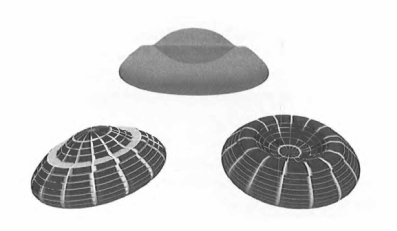
\includegraphics[width=0.8\textwidth]{imagenes/no_rigid}
	\end{center}
	\caption{Superficie no rígida.}
	\label{fig:etiq_2}
\end{figure}




\begin{definicion}
	Diremos que $S \subset \mathbb{R}^3$ es una \underline{\textbf{superficie}} si para todo $p \in S$ existe un entorno $V \subset S$ de $p$, un abierto $U \subset \mathbb{R}^2$ y una aplicación $X : U \to \mathbb{R}^3$ diferenciable tales que:
	\begin{enumerate}
		\item $X(U) = V$,
		\item la aplicación $X : U \to V$ es un homeomorfismo,
		\item $\forall q \in U$, $(dX)_q : \mathbb{R}^2 \to \mathbb{R}^3$ es inyectiva.
	\end{enumerate}
\end{definicion}
${ }$\\

\begin{teorema}
	$\textbf{(Fórmula del cambio de variable)}$ Sea $F : R_1 \to R_2$ un difeomorfismo, siendo $R_1$, $R_2$ de dos superficies orientables, y sea $\Phi : R_2 \to \mathbb{R}$ una función integrable. Entonces, $(\Phi \circ F)(p)|Jac \Phi|(p)$ es integrable y
	\[
	\int_{R_2} \Phi = \int_{R_1} (\Phi \circ F)|Jac \Phi|.
	\]
\end{teorema}
${ }$\\

\begin{teorema}\label{teo:divergencia}
	$\textbf{(Teorema de la divergencia sobre superficies)}$ Sea una superficie compacta $S$ y un campo diferenciable de vectores $V : S \to \mathbb{R}^3$. Entonces:
	\begin{enumerate}
		\item $\int_S div V = -2 \int_S \langle V, N \rangle H$,
		\item $\int_S [k_2(p) \langle (dV)_p(e_1), e_1\rangle + k_1(p) \langle (dV)_p(e_2), e_2 \rangle ] \; dp = -2 \int_S \langle V, N \rangle K$, donde $\{ e_1, e_2 \}$
	\end{enumerate}
\end{teorema}
${ }$\\

\begin{teorema} \label{teo:hadamard}
	$\textbf{(Hadamard-Stoker)}$ Sea un ovaloide $S \subset \mathbb{R}^3$ y $\Omega$ su dominio interior. Entonces:
	
	\begin{enumerate}
		\item Para todo $x, y \in \overline{\Omega}$, entonces $]x, y[ \subset \Omega$. En particular, $\Omega$ es convexo.
		\item Para cada $p \in S$, $\Pi_p \cap S = \{p\}$, donde $\Pi_p$ es el plano tangente afín a $S$ en p. Además, $\overline{\Omega} \subset \bigcap_{p \in S} \; \Pi^{+}_{p}$.
	\end{enumerate}
\end{teorema}
${ }$\\

\begin{teorema}
	$\textbf{(Fórmulas de Minkowski)}$ Sea $S$ una superficie compacta, $N$ su normal interior y $K$, $H$ sus curvaturas de Gauss y media. Entonces, se cumplen las siguientes fórmulas:
	\begin{enumerate}
		\item $\int_S (1 + \langle p, N(p) \rangle H(p) dp = 0$,
		\item $\int_S (H(p) + \langle p, N(p) \rangle K(p) dp = 0$
	\end{enumerate}
\end{teorema}
${ }$\\

(HACER UN RESPASO DE TODO LO QUE HE HECHO PARA VER QUE METO EN ESTA SECCION)


${ }$\\
${ }$\\
${ }$\\
$\textbf{RAY-MARCHING EVOLUCIÓN}$
${ }$\\

Ray-marching es una tecnica para la visualización de superficies mas complejas dadas en ecuaciones de implicitas que son las de la siguiente forma:

\[
F(x,y,z) = 0.
\]

Esta algoritmo usa el método de newton-raphson para aproximar las soluciones de una función para ir aproximandose iterativamente a la superficie. Comienza en el principio del rayo y avanza a lo largo de él la misma cantidad que la distancia de la superficie al último punto tomado.

\chapter*{Objetivos del trabajo}




\chapter*{Rigidez de ovaloides}

%\begin{definicion}\label{def:isom_loc} % label para cuando haga una referencia.
	%Dada una aplicación $f : S \longrightarrow S'$ siendo S y $S'$ dos superficies. Diremos que $f$ es \underline{\textbf{isometría local}} si $\forall$ p $\in$ S, $\exists$ V entorno de p $\exists V'$ entorno de $f(p)$ $\in S'$ tal que $f : V \longrightarrow V'$.
%\end{definicion}

%También puede definirse una isometría local como una aplicación diferenciable que cumple la primera forma fundamental. De este modo una isometría es una isometría local que es difeomorfismo. 

%Dicho esto, dos superficies son isométricas (resp. localmente isométricas) si existe un isometría (resp. isometría local) que nos lleva una superficie en la otra.

%Dicho esto, dos superficies son isométricas si existe una isometría que nos lleva una superficie en la otra.

En los siguientes dos resultados veremos que dado un movimiento rígido, su restricción a una superficie es es una isometría entre superficies que conserva la segunda forma fundamental y después veremos su reciproco, que dada una isometría entre superficies que conserva la segunda forma fundamental esta isometría se puede extender a un movimiento rígido del espacio $\mathbb{R}^3$.

\begin{proposicion}\label{prop:rig1} % label para cuando haga una referencia.
	Sean S una superficie y  $\Phi : \mathbb{R}^3 \to \mathbb{R}^3$  un movimiento rígido. Consideraremos que $S' = \Phi(S)$ y $f = \Phi_{\mid_{S}} : S \to S'$. Entonces:
	\begin{enumerate}
		\item $S'$ es una superficie y $f : S \to S'$ es un difeomorfismo.
		\item $f$ conserva la 1ª forma fundamental, esto es, $\langle df_p(u), df_p(v) \rangle $ $=$ $ \langle u, v \rangle \forall p \in S$ y $\forall u,v \in T_p S$.
		\item $f$ conserva la 2ª forma fundamental, esto es, $\sigma_p(u,v) = \sigma'_{f(p)}(df_p(u), df_p(v))$ $\forall p \in S$ y $\forall u,v \in T_p S$.
	\end{enumerate}
	%%%%%%\[ F:{\mathbb{R}_3} \to {\mathbb{R}_3} \]
\end{proposicion}

\begin{proof}
	${ }$%\\
	\begin{enumerate}
		\item Por ser $ \Phi : \mathbb{R}^3 \to \mathbb{R}^3 $ un movimiento rígido, es de la forma F(x) = Ax+b $\forall x \in \mathbb{R}^3$, con A una matriz ortogonal de orden 3 y $b \in \mathbb{R}^3$.
		
		A partir de aquí es fácil comprobar que $S'$ es una superficie. Tomando X una parametrización de $S$ basta con ver que $F\circ X$ es una parametrización de $S'$ y $f = \Phi_{\mid_{S}} : S \to S'$ es difeomorfismo.
		
		
		\item Tenemos que para todo $p \in S$ y $\forall u, v \in T_p S$
		
		\[
		(df)_p(v) = (d\Phi_{\mid S})_p(v) = (d\Phi)_p(v) = Av.
		\]
		
		De aquí podemos deducir, teniendo en cuenta que A es ortogonal y por tanto $A^{-1} = A^t$, que $f$ conserva la 1ª forma fundamental:
		\[
		<(df)_p(u), (df)_p(v)> = <Au, Av> = u^tA^tAv = <u, v>
		\]
		
		\item Sea $N : S \to \mathbb{S}^2$ una aplicación de Gauss para S y $N' : S' \to \mathbb{S}^2$ una aplicación de Gauss de la nueva superficie $S'$ definida por
		
		\[
		N'\circ f = A\circ N.
		\]
		
		Derivando obtenemos que $\forall p \in S$,  $(dN')_{f(p)}\circ A = A \circ (dN)_p$. Esto último nos permite concluir que $f$ conserva la segunda forma fundamental:
		
		\[
		\sigma'_{f(p)}((df)_p(u), (df)_p(v)) = -<(dN')_{f(p)}((df)_p(u)), (df)_p(v)>
		\]
		\[
		= -<A\circ(dN)_p(u), Av> = \sigma_p(u, v).
		\]
	\end{enumerate}
\end{proof}

\begin{teorema}
	Dadas dos superficies S y $S'$ orientables y compactas, sean N y $N'$ las aplicaciones de Gauss para sendas superficies cuyas segundas formas fundamentales asociadas son $\sigma$ y $\sigma'$ respectivamente.
	Si $f : S \to S'$ es una isometría que conserva la segunda forma fundamental, entonces existe un movimiento rígido $\Phi : \mathbb{R}^3 \to \mathbb{R}^3$ tal que $\Phi_{\mid S} = f$.
\end{teorema}

\begin{proof}
	${ }$\\
	
	Partimos de que $f$ es isometría y como S y $S'$ son compactas $\exists$ $\varepsilon > 0$ tal que $N_\varepsilon(S)$ y $N_\varepsilon(S')$ son entornos tubulares. Definimos la aplicación $\Phi$ de la siguiente forma:
	\[
	\Phi : N_\varepsilon(S) \longrightarrow N_\varepsilon(S')
	\]
	\[
	x = p + tN(p) \longmapsto f(p) + tN'(f(p))
	\]
	donde $t \in (-\varepsilon, \varepsilon)$. Entonces, $\Phi$ es biyectiva y diferenciable con inversa
	\[
	f^{-1}(q) + tN(f^{-1}(q)) \longleftarrow q + tN'(q).
	\]
	Por tanto $\Phi$ es un difeomorfismo de $N_\varepsilon(S)$ sobre $N_\varepsilon(S')$.
	
	${ }$\\	
	
	Vamos a calcular $d\Phi_{p+tN(p)}$, para ello tomamos una curva en el entorno tubular definida del siguiente modo,
	\[
	\beta(s) = \alpha(s) + tN(\alpha(s))
	\]
	donde $\alpha(S)$ es una curva contenida en S que cumple que $\alpha(0) = p$ y $\alpha'(0) = v$. Dicha curva en $s = 0$ pasa por el punto $\beta(0) = p + tN(p)$  con vector tangente $\beta'(0) = v + tdN_p(v)$. La curva así definida nos permite dar la siguiente expresión de la diferencial de $\Phi$:
	\[
	d\Phi_{(p + tN(p))}(v + tdN_p(v)) = \frac{d}{ds}_{\arrowvert_0} \Phi(\alpha(s) + tN(\alpha(s))
	\]
	\[
	= \frac{d}{ds}_{\arrowvert_0} (f(\alpha(s)) + tN'(f(\alpha(s)))) = df_p(v) + tdN'_{f(p)}(df_p(v)).
	\]
	
	%Tomando las direcciones principales ${e_1, e_2} \in T_p S$ tenemos que $dN_p(e_i) = -\lambda_ie_i$ y podemos expresar la diferencial de $\Phi$ en función de $f$ del siguiente modo:
	
	${ }$\\	
	
	Tomando las direcciones principales ${e_1, e_2} \in T_p S$ tenemos que $dN_p(e_i) = -\lambda_ie_i$ y las dos siguientes igualdades:
	\[
	d\Phi_{p + tN(p)}((1 - t\lambda_i)e_i) = df_p(e_i) + tdN'_{f(p)}(df_p(e_i)),
	\]
	
	\[
	d\Phi_{p + tN(p)}((1 - t\lambda_i)e_i) = (1 - t\lambda_i)d\Phi_{p + tN(p)}(e_i).
	\]
	
	Esto nos da una expresión de la diferencial de $\Phi$ en función de $f$,
	\[
	d\Phi_{p + tN(p)}(e_i) = \frac{1}{1 - t\lambda_i} \{df_p(e_i) + tdN'_{f(p)}(df_p(e_i))\}.
	\]
	
	Para comprobar que es isometría calculamos el producto escalar
	\[
	<d\Phi_{p + tN(p)}(e_i), d\Phi_{p + tN(p)}(e_j)> = 
	\]
	\[
	\frac{1}{(1 - t\lambda_i)(1 - t\lambda_j)}<df_p(e_i) + tdN'{f(p)}(df_p(e_i)), df_p(e_j) + tdN'{f(p)}(df_p(e_j))> =
	\]
	\[
	\frac{1}{(1 - t\lambda_i)(1 - t\lambda_j)}(<df_p(e_i), df_p(e_j)> + <df_p(e_i), tdN'_{f(p)}(df_p(e_j))> + 
	\]
	\[
	+ <df_p(e_j), tdN'_{f(p)}(df_p(e_j))> + <tdN'_{f(p)}(df_p(e_i)), tdN'{f(p)}(df_p(e_j))>\}.
	\]
	
	Como f es isometría $<df_p(e_i), df_p(e_j)> = <e_i, e_j> = \delta_{ij}$ y
	\[
	<d\Phi_{p + tN(p)}(e_i), d\Phi_{p + tN(p)}(e_j)> = \frac{1}{(1 - t\lambda_i)(1 - t\lambda_j)}\{\delta_{ij} - t\sigma'_{f(p)}(df_p(e_i), df_p(e_j)) -  
	\]
	\[
	t\sigma'_{f(p)}(df_p(e_j), df_p(e_i)) + t^2<dN'_{f(p)}(df_p(e_i)), dN'_{f(p)}(df_p(e_j))>\}.
	\]
	
	${ }$\\	
	
	Usando que f conserva la segunda forma fundamental llegamos a
	\[
	<d\Phi_{p + tN(p)}(e_i), d\Phi_{p + tN(p)}(e_j)> = \frac{1}{(1 - t\lambda_i)(1 - t\lambda_j)}\{\delta_{ij} - t\sigma_p(e_i, e_j) - 
	\]
	\[
	t\sigma_p(e_j, e_i) + t^2<dN_p(e_i), dN_p(e_j)>\} = \frac{1}{(1 - t\lambda_i)(1 - t\lambda_j)}\{\delta_{ij} - 2t(\lambda_i + \lambda_j)\delta_{ij} + t^2\lambda_i\lambda_j\delta_{ij}\}.
	\]
	
	Finalmente, sacando $\delta_{ij}$ como factor común y descomponiendo en producto de polinomios
	\[
	<d\Phi_{p + tN(p)}(e_i), d\Phi_{p + tN(p)}(e_j)> = \frac{(1 - t\lambda_i)(1 - t\lambda_j)}{(1 - t\lambda_i)(1 - t\lambda_j)}\delta_{ij} = \delta_{ij} = <e_i, e_j>.
	\]
	
	Resumiendo, acabamos de ver que
	\[
	<d\Phi_{p + tN(p)}(e_i), d\Phi_{p + tN(p)}(e_j)> = <e_i, e_j>.
	\]
	
	Tomamos ahora la curva $\alpha(s) = p + (t + s)N(p)$, con ella tenemos que
	\[
	d\Phi_{p + tN(p)}(N(p)) = \frac{d}{ds}\arrowvert_0\Phi(p + (t + s)N(p)) = \frac{d}{ds}\arrowvert_0(f(p) + (t + s)N'(f(p)) = N'(f(p))
	\]
	y ya podemos determinar que
	\[
	<d\Phi_{p + tN(p)}(e_i), d\Phi_{p + tN(p)}(N(p))> = <d\Phi_{p + tN(p)}(e_i), N'(f(p))> = 0 = <e_i, N(p)>.
	\]
	
	Por tanto, $\Phi$ es isometría de $N_\varepsilon(S)$ sobre $N_\varepsilon(S')$ y para ver que esto se traduce en un movimiento rígido haremos uso del siguiente resultado.
	
	\begin{teorema}
		Sean O y $O'$ dos subconjuntos abiertos de $\mathbb{R}^3$ y $F : O \to O'$ una isometría. Entonces $F$ se puede extender a un movimiento rígido de $\mathbb{R}^3$.
	\end{teorema}
	
	\begin{proof}
		Tenemos que
		\[
		<dF_x(u), dF_x(v)> = <u, v>, x \in O, u,v \in \mathbb{R}^3
		\]
		por ser $F$ isometría de un abierto de $\mathbb{R}^3$ en otro abierto de $\mathbb{R}^3$, y tomando que u,v son vectores de la base canónica de $\mathbb{R}^3$ se obtiene la siguiente igualdad
		\[
		<\frac{\partial F}{\partial x_i}, \frac{\partial F}{\partial x_j}> = \delta_{ij} \thinspace \thinspace \thinspace \thinspace \thinspace \thinspace \thinspace i,j = 1,2,3
		\]
		donde $x_1, x_2, x_3$ son las coordenadas de $\mathbb{R}^3$. Si derivamos con respecto a $x_k$ siendo k = 1, 2, 3, se obtenemos
		\[
		<\frac{\partial^2 F}{\partial x_i \partial x_k}, \frac{\partial F}{\partial x_j}> + <\frac{\partial^2 F}{\partial x_j \partial x_k}, \frac{\partial F}{\partial x_i}> = 0 \thinspace \thinspace \thinspace \thinspace \thinspace \thinspace \thinspace i,j = 1,2,3.
		\]
		Defiendo $G_{ijk}$ como
		\[
		G_{ijk} = <\frac{\partial^2 F}{\partial x_i \partial x_j}, \frac{\partial F}{\partial x_k}>
		\]
		este es simétrico en los i, j por el lema de Schwarz y antisimétrico tanto en los i, k como en los j, k por la igualdad que le precede. Ahora podemos operar como sigue
		\[
		G_{ijk} = -G_{ikj} = -G_{kij} = G_{kji} = G_{jki} = -G_{jik} = -G_{ijk}
		\]
		para determinar que en $O$
		\[
		<\frac{\partial^2 F}{\partial x_i \partial x_j}, \frac{\partial F}{\partial x_k}> \equiv 0
		\]
		para cada i, j, k = 1, 2, 3. Pero, como se vió al principio, las derivadas parciales $\partial F / \partial x_1$, $\partial F / \partial x_2$ y $\partial F / \partial x_3$ forman una base ortonormal de $\mathbb{R}^3$ en cada punto de $O$, por consiguiente
		\[
		\frac{\partial^2 F}{\partial x_i \partial x_j} \equiv 0
		\] en $O$, para cada  i, j = 1, 2, 3. Dicho esto y teniendo en cuenta  que $F$ es de la forma $F(x_1, x_2, x_3) = (F_1(x_1, x_2, x_3), F_2(x_1, x_2, x_3), F_3(x_1, x_2, x_3))$, sabemos que
		
		\[
		F_1(x_1, x_2, x_3) = a_{00}x_1 + a_{01}x_2 + a_{02}x_3 + b_1
		\]
		\[
		F_2(x_1, x_2, x_3) = a_{10}x_1 + a_{11}x_2 + a_{12}x_3 + b_2
		\]
		\[
		F_3(x_1, x_2, x_3) = a_{20}x_1 + a_{21}x_2 + a_{22}x_3 + b_3
		\]
		
		${ }$\\	
		
		Luego $F = Ax + b$ para cada $x \in O$, donde $A = \{a_{ij}\}_{i,j=0,1,2}$ y $b \in \mathbb{R}^3$, por ser $O$ conexo. Como $dF_x=A$ en cada $x \in O$ la matriz $A$ ha de ser ortogonal, por tanto F es la restricción a $O$ de un movimiento rígido de $\mathbb{R}^3$.
		
	\end{proof}
	
\end{proof}



\begin{ejemplo}
		Sean $P$ y $P'$ dos planos de $\mathbb{R}^3$ y $f : P \to P'$ una isometría. Ya que las formas fundamentales de ambos planos son idénticamente nulas, $f$ siempre conserva las segundas formas fundamentales. Por tanto $f$ se puede extender a un movimiento rígido.
\end{ejemplo}

\begin{ejemplo}
	Sean S y S' dos esferas con el mismo radio y sea $f : S \to S'$ una isometría. La segunda forma fundamental, en cada punto, de ambas superficies está expresada como $-\frac{1}{r}<v,w>$ para cada v, w de sus respectivos tangentes, por tanto $f$ conserva la segunda forma fundamental y se puede extender a un movimiento rígido.
\end{ejemplo}

\begin{teorema}
	$\textbf{(Teorema Egregium)}$ Sean $f : S \to S'$ una isometría local entre dos superficies y K y K' sus respectivas curvaturas de Gauss. Entonces, $K = K'\circ f$.
\end{teorema}

\begin{proof}
	${ }$\\
	Tomemos una parametrización $X : U \to S$, entonces $X_u, X_v$ nos dan una base del plano tangente y $N^X = \frac{X_u \wedge X_v}{|X_u \wedge X_v|} : U \to \mathbb{R}^3$.
	
	Antes de la demostración del teorema probaremos que la siguiente igualdad es cierta en las condiciones que se especifican:
	\begin{lema}
		Sean un abierto de $U$ de $\mathbb{R}^3$ y una aplicación $X : U \to S$ diferenciable como lo son las parametrizaciones de una superficie. Si llamamos $K$ a la curvatura de Gauss de $S$ se cumple la siguiente igualdad en los puntos de $U$,
		\[
			<({X^T}_{vv})_u - ({X^T}_{uv})_v, X_u> = (K \circ F)(|X_u|^2|X_v|^2 - <X_u, X_v>^2),
		\]
		donde el superíndice T indica que te toma la parte del vector que está en el plano tangente a la superficie.
	\end{lema}
	\begin{proof}
		\[
			X_{uv} = {X^T}_{uv} + <X_{uv}, N^X>N^X = {X^T}_{uv} + (<X_u,N^X>_v - <X_u, {N^X}_v>)N^X,
		\]
		\[
			X_{vv} = {X^T}_{vv} + <X_{vv}, N^X>N^X = {X^T}_{vv} + (<X_v,N^X>_v - <X_v, {N^X}_v>)N^X.
		\]
		
		Despejando en ambas igualdades
		
		\[
			{X^T}_{uv} = X_{uv} + <X_u, {N^X}_v>N^X,
		\]
		\[
			{X^T}_{vv} = X_{vv} + <X_v, {N^X}_v>N^X.
		\]
		
		Derivando en $v$ y en $u$ respectivamente
		
		\[
			({X^T}_{uv})_v = X_{uvv} + <X_u, {N^X}_v>_v N^X + <X_u, {N^X}_v> {N^X}_v,
		\]
		\[
			({X^T}_{vv})_u = X_{vvu} + <X_v, {N^X}_v>_u N^X + <X_v, {N^X}_v>{N^X}_u.
		\]
		
		Hacemos el producto escalar de estas dos últimas expresiones por $X_u$ y las restamos
		
		\[
			<({X^T}_{uv})_v, X_u> = <X_{uvv}, X_u> + <X_u, {N^X}_v>^2,
		\]
		\[
			<({X^T}_{vv})_u, X_u> = <X_{vvu}, X_u> + <X_v, {N^X}_v><{N^X}_u, X_u>,
		\]
	${ }$\\	
		\[
			<({X^T}_{vv})_u, X_u> - <({X^T}_{uv})_v, X_u> = <X_v, {N^X}_v><{N^X}_u, X_u> - <X_u, {N^X}_v>^2
		\]
		\[
			= eg - f^2.
		\]
		
		Donde,
		
		\[
			e = \sigma(X_u, X_u) = - <dN(X_u), X_u> = - <d(N\circ X)(\frac{\partial}{\partial u} ), X_u> =
		\]
		\[
			= - <dN^X(\frac{\partial}{\partial u} ), X_u> = - <{N^X}_u, X_u>
		\]
	${ }$\\	
		\[
			g = \sigma (X_v, X_v) =  - <{N^X}_v, X_v> \;\;\;\;\;\;\;\;\;\;\;\; f = \sigma (X_v, X_u) =  - <{N^X}_v, X_u>
		\]
		
		Por tanto, usando que la curvatura de Gauss es
		
		\[
			K \circ X = \frac{eg - f^2}{|X_u|^2|X_v|^2 - <X_u, X_v>^2}
		\]
		obtenemos el resultado.

	\end{proof}
	
	
	Para la demostración del Tª Egregium aplicamos el lema demostrado anteriormente a la parametrización $X$, teniendo así
	
	\[
		<({X^T}_{vv})_u - ({X^T}_{uv})_v, X_u> = (K \circ F)(EG - F^2),
	\]
	
	Tambien tenemos que $X' = f \circ X$ es una parametrización de la superficie $S'$. Aplicando el lema a la segunda superficie tenemos
	
	\[
		<({X'^T}_{vv})_u - ({X'^T}_{uv})_v, X'_u> = (K' \circ F')(E'G' - F'^2),
	\]
	
	Por otro lado, calculando las derivadas parciales de $X'$ mediante la regla de la cadena, tenemos
	
	\[
		X'_u = (df)_X(X_u) \;\;\;\;\;\; y \;\;\;\;\;\; X'_v = (df)_X(X_v).
	\]
	
	Usando que f es isometría local, tenemos
	
	\[
		E' = |X'_u|^2 = |(df)_X(X_u)|^2 = |X_u|^2 = E
	\]
	
	\[
		G' = |X'_v|^2 = |(df)_X(X_v)|^2 = |X_v|^2 = G.
	\]
	
	\[
		F' = <X'_u, X'_v> = <(df)_X(X_u), (df)_X(X_v)> = <X_u, X_v> = F
	\]
	
	Derivando $E$ y $G$ con respecto a $u$ y $v$, tenemos
	
	\[
		<X_{uv}, X_u> = <X'_{uv}, X'_u> \;\;\;\;\;\;  \;\;\;\;\;\; <X_{uu}, X_u> = <X'_{uu}, X'_u>,
	\]
	
	\[
		<X_{vu}, X_v> = <X'_{vu}, X'_v> \;\;\;\;\;\;  \;\;\;\;\;\; <X_{vv}, X_v> = <X'_{vv}, X'_v>.
	\]
	
	Derivando tambien $F$ con respecto a $u$ y $v$, obtenemos
	
	\[
		<X_{uu}, X_v> + <X_u, X_{vu}> = <X'_{uu}, X'_v> + <X'_u, X'_{vu}>
	\]
	
	\[
		\to <X_{uu}, X_v> = <X'_{uu}, X'_v>
	\]
	
	\[
		<X_{uv}, X_v> + <X_u, X_{vv}> = <X'_{uv}, X'_v> + <X'_u, X'_{vv}>
	\]
	
	\[
		\to <X_u, X_{vv}> = <X'_u, X'_{vv}>
	\]
	
	Considerando
	
	\[
		{X^T}_{vv} = AX_u + BX_v
	\]
	
	\[
		<X_{vv}, X_u> = A|X_u|^2 + B<X_u, X_v> \;\;\;\;\;\; <X_{vv}, X_v> = A<X_u, X_v> + B|X_v|^2
	\]
	
	\[
		{X'^T}_{vv} = A'X'_u + B'X'_v
	\]
	
	\[
		<X'_{vv}, X'_u> = A'|X'_u|^2 + B'<X'_u, X'_v> \;\;\;\;\;\; <X'_{vv}, X'_v> = A'<X'_u, X'_v> + B'|X'_v|^2
	\]
	obtenemos que
	
	\[
		A = A' \;\;\;\;\;\; y \;\;\;\;\;\; B = B',
	\]
	de aquí seguimos que
	
	\[
		(df)_X(X^{T}_{vv}) = A(df)_X(X_u) + B(df)_X(X_v) = AX'_u + BX'_v = X^{'T}_{vv},
	\]
	análogamente tenemos
	\[
		(df)_X(X^{T}_{uv}) = X^{'T}_{uv}.
	\]
	
	Finalmente comprobamos que
	
	\[
		<(X'^{T}_{vv})_u, X'_u> = <(X'^{T}_{vv}), X'_u>_u - <(X'^{T}_{vv}), X'_{uu}>
	\]
	
	\[
		= <(df)_X(X^{T}_{vv}), (df)_X(X_u)>_u - <(df)_X(X^{T}_{vv}), (df)_X(X_{uu})>
	\]
	
	\[
		= <X^{T}_{vv}, X_u>_u - <X^{T}_{vv}, X_{uu}> = <(X^{T}_{vv})_u, X_u>
	\]
	por un procedimiento análogo, tenemos que
	
	\[
		<(X'^{T}_{uv})_v, X'_u> = <(X^{T}_{uv})_u, X_u>.
	\]
	${ }$\\	
	
	Entonces,
	
	\[
		K \circ X = K' \circ X' = K' \circ f \circ X,
	\]
	de donde se desprende que   $\;\; K = K' \circ f$.
	
\end{proof}

\begin{teorema}
	$\textbf{(Rigidez de la esfera)}$ Consideremos una esfera de radio $r>0$, $\mathbb{S}^2(r)$, y $S$ una superficie conexa cualquiera. En esta situación toda isometría $f : \mathbb{S}^2(r) \to S$ es la restricción de un movimiento rígido de $\mathbb{R}^3$. En particular, $S$ es una esfera de igual radio que la de partida.
\end{teorema}

\begin{proof}
	Por ser $f$ isometría es también difeomorfismo y por ende es una aplicación abierta. Por tanto, su imagen $f(\mathbb{S}^2(r))$ es un abierto de $S$. Además es un cerrado por ser imagen de un compacto $(\mathbb{S}^2(r))$ en un espacio Hausdorff.
	
	Finalmente, por el teorema Egregium concluimos la demostración.
\end{proof}
	${ }$\\
%Como acabamos de ver la rigidez es una propiedad de las esferas, aunque no es exclusiva para las esferas sino para mas superficies entre ellas los ovaloides (como veremos mas adelante). Sin embargo, hay superficies que no tienen esta propiedad de rigidez como se puede observar en el ejemplo que se muestra en la Figura \ref{fig:etiq_2}

Supongamos ahora dos superficies $S$ y $S'$ orientables  y $f : S \to S'$ una isometría entre ellas. Si $V : S \to \mathbb{R}^3$ es un campo diferenciable de vectores tangentes a la superficie $S$, entonces definimos otro campo tangente a $S$ por

	\[
		W(p) = A(f)_p(V(p)), \;\;\; p \in S.
	\]
Donde $A(f)_p : T_p S \to T_p S$ para $p \in S$ se define como el endomorfismo lineal

	\[
		A(f)_p = -(df)^{-1}_{p} \circ (dN')_{f(p)} \circ (df)_p
	\]
y $N'$ es la aplicación de Gauss de $S'$.

\begin{lema} \label{lem:lema1}
	En las condiciones especificadas anteriormente:
	\begin{enumerate}
		\item $W$ es un campo diferenciable.
		\item La divergencia de $W$ viene dada por 
		\[
			(div W)(p) = 2 \langle \nabla (H' \circ f)(p), V(p) \rangle + \sum_{i=1}^{2} \lambda'_{i}(f(p)) \langle dV_p(e_i), e_i \rangle.
		\]
	\end{enumerate}
	
\end{lema}


	${ }$\\
	
	Para la demostración de este resultado será necesario recordar lo que se enuncia en la siguiente proposición.
	${ }$\\
	
	\begin{proposicion}
		Sea $X : U \subset \mathbb{R}^2 \to S$ una parametrización de S, la aplicación lineal $dN_X : T_X S \to T_X S$ viene dada en la base $\{X_u, X_v \}$ como
		\[
			dN_X = - \left( {\begin{array}{cc}
						E & F \\
						F & G \\
					\end{array} } \right)^{-1}
					\left( {\begin{array}{cc}
						e & f \\
						f & g \\
					\end{array} } \right)
		\]
		y por tanto la curvatura media esta dada por
		\[
			H \circ X = \frac{eG + gE -2fF}{2(GE-F^2)}.
		\]
		
		Además, fijando un punto $p \in S$ se puede encontrar una parametrización con $(0,0) \in U$ tal que:
		\begin{enumerate}
			\item $\{X_u(0,0), X_v(0,0) \}$ es una base ortonormal de $T_p S$.
			\item Las derivadas de $E$, $G$, y $F$ respecto de $u$ y $v$ se anulan en (0,0).
			\item $e(0,0) = \lambda_{1}(p)$, $g(0,0) = \lambda_{2}(p)$ y $f(0,0) = 0$, donde los $\lambda_i$ son las curvaturas principales.
			\item Se cumple que $e_v(0,0) = f_u(0,0)$ y $g_u(0,0) = f_v(0,0)$.
		\end{enumerate}
		
		Recordemos además que $E = \langle X_u, X_u \rangle$, $G = \langle X_v, X_v \rangle$ y $F = \langle X_u, X_v \rangle$. $N \circ X = \frac{X_u \times X_v}{\sqrt{EG-F^2}}$ y $e = \sigma_X(X_u, X_u)$, $g = \sigma_X(X_v, X_v)$ y $f = \sigma_X(X_u, X_v)$.
	\end{proposicion}
	${ }$
\begin{proof}	
	${ }$\\
	
	(1)  Sea $X : U \subset \mathbb{R}^2 \to S$ una parametrización de $S$ sabemos que $X' = f \circ X$ es una parametrización de $S'$ definida también en $U$. Además, debido a que $df_X(X_u) = X'_{u}$ y $df_X(X_v) = X'_{v}$ se tiene que $df_X$ y $(df_X)^{-1}$ son la identidad cuando están definidas en las bases $\{X_u, X_v \}$ y $\{X'_{u}, X'_{v} \}$. Es por eso, que la aplicación lineal $A(f)^X = A(f)_X = -(df)^{-1}_{X} \circ (dN')_{X'} \circ (df)_X$ en la base $\{X_u, X_v \}$ viene dada por la matriz $-(dN')_{X'}$ en la base $\{X'_{u}, X'_{v} \}$ por
	
	\[
		A(f)_X = \left( {\begin{array}{cc}
			E' & F' \\
			F' & G' \\
			\end{array} } \right)^{-1}
		\left( {\begin{array}{cc}
			e' & f' \\
			f' & g' \\
			\end{array} } \right).
	\]
	${ }$\\
	
	Si $V^X = V \circ X$ y $W^X = W \circ X$, entonces $V^X = aX_u + bX_v$, para $a,b$ definidas en $U$. Por tanto, $W^X = mX_u + nX_v$, donde
	
	\[
		\left( {\begin{array}{c}
			m \\
			n \\
			\end{array} } \right)
		=
		\left( {\begin{array}{cc}
			E' & F' \\
			F' & G' \\
			\end{array} } \right)^{-1}
		\left( {\begin{array}{cc}
			e' & f' \\
			f' & g' \\
			\end{array} } \right)
		\left( {\begin{array}{c}
			a \\
			b \\
			\end{array} } \right).
	\]
	De aquí se deduce que $m$ y $n$ son diferenciables y por lo tanto $W^X$ también lo es.
	${ }$\\
	
	(2)  Sea $p \in S$, entonces
	
	\[
		(div W)(p) = \sum_{i=1}^{2}\langle dW_p(e_i), e_i \rangle,
	\]
	donde $\{e_1, e_2\}$ es una base ortonormal de $T_p S$.
	${ }$\\
	
	Tomamos $X'$ una parametrización de $S'$ alrededor de $f(p)$, con $X'(0,0) = f(p)$, la cual cumpla las propiedades de la proposición anterior. Si tomamos $X = f^{-1} \circ X'$ se pueden usar las expresiones de $m$ y $n$ que hemos visto y ya que $f$ es isometría la parametrización $X$ cumple las propiedades 1 y 2 de la proposición. La proposición anterior también nos permite tomar $e_1 = X_u(0,0)$ y $e_2 = X_v(0,0)$. Por tanto, se tiene que
	
		\begin{eqnarray*}
		(\hbox{div}\,W)(p)&=&\langle W^X_u,X_u\rangle(0,0)+\langle W^X_v,X_v\rangle(0,0)\\
		&=&\langle m_uX_u+mX_{uu}+n_uX_v+nX_{vu},X_u\rangle(0,0)\\
		&+&\langle m_vX_u+mX_{uv}+n_vX_v+nX_{vv},X_v\rangle(0,0)\\
		&=&(m_u+n_v)(0,0).
		\end{eqnarray*}
	${ }$\\
	
	Haciendo los cálculos de la expresión matricial vista anteriormente obtenemos
	${ }$\\
	
	\[
		m = \frac{1}{E'G' - F'^2} (G'(ae' + bf') - F'(af' + bg')),
	\]
	\[
		n = \frac{1}{E'G' - F'^2} (-F'(ae' + bf') + G'(af' + bg')).
	\]
	
	Así, derivando las dos expresiones anteriores y aplicando en el resultado el apartado 4 de la proposición, llegamos a que
	\begin{eqnarray*}
		(\hbox{div}\,W)(p)&=&(ae'+bf')_u(0,0)+(af'+bg')_v(0,0)\\
		&=& a_ue'(0,0)+ae'_u(0,0)+bf'_u(0,0)+af'_v(0,0)+b_vg'(0,0)+bg'_v(0,0)\\
		&=& (a_ue'+b_vg')(0,0)+a(e'_u+g'_u)(0,0)+b(e'_v+g'_v)(0,0).
	\end{eqnarray*}
	
	Usando 3 de la proposición, se tiene
	\[
		(H' \circ X')_u (0,0) = \frac{(e'_{u} + g'_{u})(0,0)}{2}, \;\;\; (H' \circ X')_v (0,0) = \frac{(e'_{v} + g'_{v})(0,0)}{2},
	\]
	${ }$\\
	de donde finalmente se puede concluir
	
	\begin{eqnarray*}
		(\hbox{div}\,W)(p)&=& \langle V^X_u,X_u\rangle(0,0) \lambda'_1(f(p))+\langle V^X_v,X_v\rangle(0,0) \lambda'_2(f(p))\\ &+& 2\langle V^X,X_u\rangle(0,0)(H'\circ X')_u(0,0)+2\langle V^X,X_v\rangle(0,0)(H'\circ X')_v(0,0)\\
		&=&\sum_{i=1}^2\langle dV_p(e_i),e_i\rangle\lambda'_i(f(p))+2\sum_{i=1}^2\langle V(p),e_i\rangle d(H'\circ f)_p(e_i)\\
		&=&\sum_{i=1}^2\langle dV_p(e_i),e_i\rangle\lambda'_i(f(p))+2\langle V(p),\nabla(H'\circ f)(p)\rangle.
	\end{eqnarray*}
\end{proof}
${ }$\\

\begin{teorema}\label{teo:herglotz}
	$\textbf{(Fórmula integral de Herglotz)}$
\end{teorema}


\begin{proof}
	${ }$\\
	
Del apartado 2) del lema anterior  \ref{lem:lema1} y usando el primer apartado del teorema de la divergencia para superficies \ref{teo:divergencia}

\[
	2 \int_S \langle \nabla (H' \circ f)(p), V(p) \rangle + \int_S \sum_{i=1}^{2} \lambda'_{i}(f(p)) \langle dV_p(e_i), e_i \rangle = \int_S (div W)(p) = 
\]
\[
	= -2 \int_S \langle W, N \rangle H = -2 \int \langle mX_u + nX_v, N \rangle H = 0
\]

Tomando ahora el campo $V : S \to \mathbb{R}^3$ definido de la siguiente forma
\[
	V(p) = P^T = p - \langle p, N(p) \rangle N(p) \;\;\; p \in S,
\]
siendo N la aplicación de Gauss de la superficie S. Derivando y haciendo el tangente obtenemos
\[
	(dV)_p(v)^T = v - \langle p, N(p) \rangle (dN)_p(v) -N(\langle p, N(p) \rangle N(p),
\]
de aquí y teniendo en cuenta que $N$ es perpendicular a $X_u$ y $X_v$, se tiene que
\[
	\sum^{2}_{i=1} \langle dV_p (e_i), e_i \rangle (K_{i}' \circ f)(p) = \sum^{2}_{i=1} \{ 1 - \langle p, N(p) \rangle \langle dN_p(e_i), e_i \rangle \} (K_{i}' \circ f)(p) = 
\]
\[
	2 (H' \circ f)(p) - \langle p, N(p) \rangle Traza (dN)_p A(f)_p
\]
y por la proposición anterior obtenemos
\[
	2 \int_S \langle \Delta (H' \circ f)_p, p \rangle \; dp = -2 \int_S (H' \circ f)(p) \; dp + \int_S \langle p, N(p) \rangle Traza (dN)_p A(f)_p \; dp
\]
\end{proof}
${ }$\\






\begin{teorema}
	$\textbf{(Rigidez de Cohn-Vossen)}$ Sean $S$ y $S'$ ovaloides. Entonces, cualquier isometría $f : S \to S'$ es restricción de un movimiento rígido.
\end{teorema}

\begin{proof}
	Como la aplicación f es un difeomorfismo, con ella podemos contruir el siguiente endomorfismo simétrico
	\[
		A(f)_p = -(df)^{-1}_{p} \circ (dN')_{f(p)} \circ (df)_p, \;\;\; p \in S
	\]
	este endormorfismo tiene traza $2(H' \circ f)$ y determinante $K' \circ f$. Ahora podemos usar el Teorema Egregium de Gauss, ya que f es isometría local, obteniendo
	
	\[
		det A(f) = K' \circ f = K.
	\]
	Además por la fórmula de Minkowski tenemos
	\[
		2 \int_S H = -2 \int_S \langle p, N(p) \rangle K(p) dp
	\]
	\[
		= - \int_S \langle p, N(p) \rangle det(dN)_p dp - \int_S \langle p, N(p) \rangle det A(f)_p dp.
	\]
	y restando por la fórmula integral de Herglotz que era
	\[
		2 \int_S H' \circ f = \int_S \langle p, N(p) \rangle [traza(dN)_p trazaA(f)_p - traza(dN)_p A(f)_p] dp,
	\]
	obtenemos
	\[
		2 \int_S (H' \circ f - H)(p) dp = \int_S \langle p, N(p) \rangle det[A(f)_p + (dN)_p] dp,
	\]
	ya que $traza(dN)_p trazaA(f)_p - traza(dN)_p A(f)_p + det(dN)_p + det A(f)_p = det[A(f)_p + (dN)_p]$ como podemos ver en el siguiente lema ya que $(dN)_p$ y $A(f)_p$ son dos endomorfismos autoadjuntos.
${ }$\\

	\begin{lema}
		Sean $\Phi$ y $\Psi$ dos endormorfismos autoadjuntos de un plano vectorial euclídeo. Entonces, $traza \Phi traza\Psi - traza \Phi \circ \Psi + det \Phi + det \Psi = det (\Phi + \Psi)$
	\end{lema}
	
	\begin{proof}
		Como $\Phi$ es autoadjunto en un espacio de dimensión finita, entonces existe una base ortonormal de $V$, un plano vectorial euclídeo donde $\Phi$ está definido, que lo diagonaliza.
		
		Pongamos que $\lambda_1$ y $\lambda_2$ son sus valores propios, al ser $\Psi$ también autoadjunto, podemos expresar $\Phi$ y $\Psi$ matricialmente como sigue
		
		\[
			\Phi = \left( {\begin{array}{cc}
				\lambda_1 & 0 \\
				0 & \lambda_2 \\
				\end{array} } \right),
			\;\;\;\;\;
			\Psi = \left( {\begin{array}{cc}
				a & b \\
				b & c \\
				\end{array} } \right), \;\;\;\;\; a, b,c \in \mathbb{R}.
		\]
		
		Se prueba el resultado haciendo los debidos cálculos con las matrices de $\Phi$ y $\Psi$ que acabamos de mostrar.
	\end{proof}
	
	Una vez tenemos todo esto queremos probar que $f$ es restricción de un movimiento rígido comprobando que se conservan las segundas formas fundamentales lo cual es equivalente a probar que $(dN')_{f(p)} \circ (df)_p = (df)_p \circ (dN)_p$, esto se obtiene cuando
	\[
		2\int_S (H' \circ f - H)(p) dp = 0,
	\]
	ya que entonces $A(f)_p = -(dN)_p$ en todo $p \in S$.
	
	Vamos probar que se anula viendo primero que tiene que ser mayor o igual a 0 y despues veremos que también debe ser menor o igual a 0.
	
	\[
		\int_S (H' \circ f - H)(p) \; dp = \int_S \langle p, N(p) \rangle det[A(f)_p + (dN)_p] \; dp \geq 0,
	\]
	ya que como veremos ahora la función soporte es negativa y el determinante de $A(f)_p + (dN)_p$ es menor o igual que cero.
	
	\begin{observacion}
		Si $p \in S$, del apartado 2) de el teorema \ref{teo:hadamard} de Hadamard-Stocker se deduce
		\[
			h_p (q) = \langle p - q, N(p \rangle) \geq 0, \;\;\;\;\;\; \forall q \in \Omega,
		\]
		ya que la igualdad se cumple cuando $q = p$.
		
		Por tanto, la función soporte de S asociada al normal interior es siempre negativa.
	\end{observacion}
	
	\begin{lema}
		Sean $\Phi$ y $\Psi$ dos endomorfismos autoadjuntos definidos positivos o negativos de un plano vectorial euclídeo y $det \Phi = det \Psi$. Entonces, $det (\Phi + \Psi) \leq 0$ y la igualdad se da si y solo si $\Phi = - \Psi$.
	\end{lema}
	\begin{proof}
		Supongamos que $det(\Phi + \Psi) > 0$, y tomemos como $ {v_1 , v_2} $ una base que diagonaliza a $\Phi + \Psi$ entonces podemos expresarlo como
		\[
			\Phi + \Psi = \left( {\begin{array}{cc}
									\mu_1 & 0 \\
									0 & \mu_2 \\
								\end{array} } \right).
		\]
		
		entonces $\Phi - \Psi$ es definido positivo. Si tomamos una base que diagonalize a $\Phi$ dada por $\{e_1, e_2\}$, tenemos
		\[
			\langle \Phi(e_i), e_i \rangle - \langle \Psi(e_i), e_i \rangle > 0, \;\;\;\; para \;\; i = 1,2.
		\]
		
		TERMINAR....
		
	\end{proof}
	
	Finalmente, para la otra desigualdad tomamos $f^{-1}$ siendo su dominio $S'$ tenemos
	\[
		\int_{S'} (H \circ f^{-1} - H')(p) \; dp \geq 0,
	\]
	a lo cual aplicamos la fórmula del cambio de variable para $f$ cuyo jacobiano tiene determinante igual a 1 por ser isometría, llegando así a
	\[
		\int_S (H - H' \circ f) (p) \; dp \geq 0
	\]
\end{proof}

\chapter*{Ray-Tracing}

$\textbf{INTRODUCCIÓN}$
${ }$\\

Antes de comenzar con Ray-Marching empezaré implementando un pequeño algoritmo de Ray-Tracing sobre el que implementaré luego el algoritmo Ray-Marching. Esta primera implementación incluirá la visualización de superficies en 3D con iluminación sencilla y sin texturas, solo con colores mate. Para probar la implementación se creará una escena con un cubo y una esfera.

${ }$\\
$\textbf{RAY-TRACING}$
${ }$\\
%%%Explicar Ray-Tracing con alguna imagen

La forma de almacenar la información se llevará a cabo mediante una matriz de tantas filas y columnas como filas y columnas de pixeles tenga la ventana donde se va a visualizar la escena. Cada elemento de esta matriz almacenará el color del correspondiente pixel.
	${ }$\\	
	
El color de cada pixel se representará mediante una tupla de tres valores \textbf{double} que se corresponderán los colores rojo, azul y verde (esta representación codificación del color se llama RGB). El valor \textbf{double} que irá de 0.0 a 1.0 indicará la cantidad de ese color.
	${ }$\\	
	
Los rayos y las superficies serán representadas mediante sus expresiones matemáticas. Determinaremos el color de cada pixel mediante el cálculo de la intersección de una recta con la superficie, cada rayo se corresponderá con uno de los pixeles siendo el valor del pixel el color de la superficie del punto donde interseca el rayo (en el caso de que tenga puntos de intersección con la superficie). Para ilustrar como se corresponden los pixeles con los rayos solo basta imaginar una matriz (como un trozo de plano dividido en el espacio), frente a la escena que se quiere visualizar y hacer que de cada elemento de la matriz salga un rayo perpendicular a dicho plano.
	${ }$\\	
	
El color del punto se determina teniendo en cuenta el color de la superficie en dicho punto y, añadiendo la iluminación, también se considerará el ángulo que forma la fuente de iluminación con la normal del objeto en ese punto y el color de la fuente de luz como indica la Ley de Lambert que se verá más adelante.
	${ }$\\	
%%% Hablar de que están implementados los operadores con tuplas3f, producto escalar etc...

En este caso para visualizar la escena se va a utilizar un simulador de cámara estenopeica. Podemos ver una cámara esteopeica en la Figura \ref{fig:etiq_1}. Este mecanismo de captura de imágenes consiste en una caja cuyo interior es de color negro con un agujero en un lateral y material fotosensible que capturará la imagen en el lateral opuesto.
	${ }$\\	

%%% Imagen Pinhole camera

\begin{figure}
	\begin{center}
		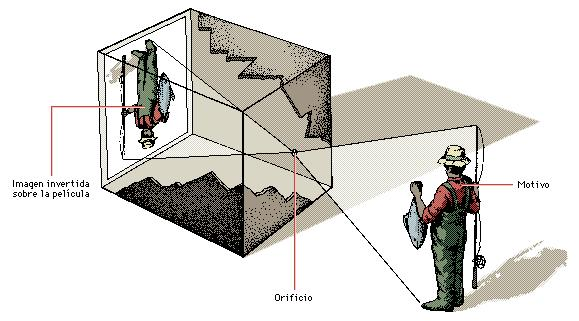
\includegraphics[width=0.6\textwidth]{imagenes/camara-estenopeica.jpg}
	\end{center}
	\caption{Cámara estenopeica}
	\label{fig:etiq_1}
\end{figure}

Primero consideraremos el sistema de referencia de visualización el cual está definido por un punto de origen \textbf{o} y una base ortonormal \{$\textbf{u}$, $\textbf{v}$, $\textbf{w}$\}. Para implementar la cámara, se tomará un rectángulo en el espacio que estará alineado con los ejes $\textbf{u}$ y $\textbf{v}$ como se muestra en la Figura\ref{fig:etiq_3}, este rectángulo se encuentra a distancia $\textbf{s}$ del origen $\textbf{o}$. Llamaremos $\textbf{a}$ y $\textbf{b}$ a las esquinas del rectangulo, que vienen dadas en coordenadas sobre la base \{$\textbf{u}$, $\textbf{v}$, $\textbf{w}$\}.
	${ }$\\

% Imagen propia 1
\begin{figure}
	\begin{center}
		
\includegraphics[width=1.1\textwidth]{imagenes/Imagen1.jpg}
	\end{center}
	\caption{Cálculo de los rayos de visión.}
	\label{fig:etiq_3}
\end{figure}



%%% Hacer yo una imagen con el sistema de coordenadas y el rectangulo dividido con los rayos saliendo del punto.

Sobre el rectángulo tomaremos muestras que se corresponderán con los pixeles que ocupa la ventana de visualización. Imaginemos que el rectángulo está dividido en tantas filas y columnas como filas-1 y columnas-1 de pixeles necesitamos para crear la imagen. La forma de tomar el valor para estas muestras se llevará a cabo mediante rayos que pasan por $\textbf{o}$ y por las intersecciones de los segmentos que hemos usado para las divisiones que hemos trazado antes sobre el rectángulo (incluyendo los propios segmentos del rectángulo). Las coordenadas de puntos intersección de segmentos dicha se calculan mediante los siguientes cálculos, estas coordenadas están dadas en la base \{$\textbf{u}$, $\textbf{v}$\}
	${ }$\\
	${ }$\\
	${ }$\\


\[
	u_i = a_1 + (b_1-a_1) \frac{i}{n_x-1}, \;\;\; 0 \leq i \leq n_x -1,
\]

\[
	v_j = a_2 + (b_2-a_2) \frac{j}{n_y-1}, \;\;\; 0 \leq j \leq n_y -1.
\]

Entonces los rayos que nos interesan se expresan del siguiente modo en el sistema de referencia de visualización:

\[
	p_{i,j}(t) = (0,0,0) + t(u_i , v_j, -s).
\]

En las coordenadas del espacio, en las que está expresada la superficie, esto se traduce en 

\[
	p_{i,j}(t) = e + t( u_i \; u, v_j \; v, -s \; w).
\]

Para poder establecer el punto \textbf{o} de visión y la orientación se calcula el sistema de referencia de visión del siguiente modo:
\begin{itemize}
	\item \textbf{o} : Será el que hemos visto hasta ahora, el punto de visión (donde se encuentra el observador) dado en coordenadas del espacio $xyz$.
	\item \textbf{g} : Se define como un vector en las coordenadas $xyz$ que indica la dirección en la que el observador mira.
	\item \textbf{$v_{up}$} : es un vector que apunta hacia arriba (hacia donde nosotros queramos que sea arriba en la imagen).
	\item \textbf{s} : la distancia de \textbf{o} al rectángulo de visión.
	\item \textbf{a}, \textbf{b} : los que hemos visto con anterioridad, son las esquinas del rectángulo de visión en la base \{$\textbf{u}$, $\textbf{v}$, $\textbf{w}$\}
\end{itemize}

Con estos datos los vectores de la base ortonormal de visión son
	\[
		w = - \frac{g}{\parallel g \parallel},
	\]
	\[
		u = \frac{v_{up} \times w}{\parallel v_{up} \times w \parallel},
	\]
	
	\[
		v = w \times u.
	\]
	
Si queremos que el rectángulo de visión este centrado con respecto a g hay que asegurarse de que $a_1 = -b_1$ y $a_2 = -b_2$. Además, si no queremos que la imagen resultante se vea estirada en alguno de los ejes \textbf{u} o \textbf{v} debemos asegurarnos de las que divisiones realizadas sobre el rectángulo de visión sean del mismo tamaño tanto para las filas como para las columnas quedandando dividido el rectángulo en cuadrados, esto se consigue asegurandose de que
	\[
		\frac{b_1-a_1}{b_2 - a_2} = \frac{n_x}{n_y}.
	\]
	${ }$\\

En el siguiente código la función $TFG\_Image$ se encarga de devolver la imagen que se ve desde el punto del observador en una matriz de dimensiones iguales a las del tamaño de la ventana donde se muestra la imagen, la funión $interposicionObjeto$ y la Ley de Lambert se verán mas adelante en la parte de iluminación. La función $TFG\_Inicializar$ se encarga de inicializar los objetos de la escena y otras variables necesarias para la visualización.
%%%[style=Consola]
\begin{lstlisting}[style=Consola]
vector<Objeto *> objetos;

float a1, a2, b1, b2;
float s = 6.0;
Tupla3f e = Tupla3f(0,0,8);
Tupla3f g = Tupla3f(0,0,-2);
Tupla3f vup = Tupla3f(0,1,0);
Tupla3f u, v, w;

LuzDireccional luz = LuzDireccional(Tupla3f(1.5,1.5,1.65), Tupla3f(1, 1, 1));


void TFG_Inicializar(int x, int y) {

  //Inicializacion de los objetos de la escena

  objetos.push_back(new Esfera(Tupla3f(0,0,0), 2.0, Tupla3f(0.3, 0.3, 0.3)));
  objetos.push_back(new Cubo(Tupla3f(1.5,1.5,1.5), Tupla3f(2,2,2), Tupla3f(0.5, 0.5, 0.5)));
  objetos.push_back(new Esfera(Tupla3f(-1.5,-1.5,1.5), 0.5, Tupla3f(0.55, 0.55, 0.55)));



  //Inicializacion de los elementos de la vista

  //Nos aseguramos de que la imagen no aparezca ensanchada
  a1=-x/200.0;
  a2=y/200.0;
  b1=-a1;
  b2=-a2;

  //Calculamos la base de visualizacion
  w = (-1)*normalized(g);
  u = normalized(vup*w);
  v = w*u;
}
\end{lstlisting}



\begin{lstlisting}[style=Consola]
Tupla3f* TFG_Image(int x, int y){
  //Direccion de los rayos de vision y matriz que contiene a la imagen
  Tupla3f direccion;
  Tupla3f *image = new Tupla3f [x*y];

  for(int i = 0; i < x; i++) {
    for (int j = 0; j < y; j++){
      direccion = (a1 + (b1 - a1)*(i/(x-1.0)))*u + (a2 + (b2 - a2)*(j/(y-1.0)))*v -s*w;


      if (!objetos.empty()){

        int indice_min;
        double int_ant;

        primeraInterseccion(direccion, int_ant, indice_min);

        if (int_ant >= 0) {
          image[i*y +j] = luz.LeyLambert( (objetos[indice_min])->getColor(), (objetos[indice_min])->normal(e, direccion, int_ant));
          if (interposicionObjeto(direccion, int_ant, indice_min) == true) image[i*y +j] = Tupla3f(0, 0, 0);
        }	
        else image[i*y +j] = Tupla3f(1, 1, 1);
      }
    }
  }
  return image;
}

\end{lstlisting}
${ }$\\

Cuando hay varios objetos en la escena hay que tener en cuenta cual es el primero que se encuentra el rayo en su recorrido esto se implementa en la siguite función.

\begin{lstlisting}[style=Consola]

void primeraInterseccion(Tupla3f direccion, double &min_inter, int &indice_min){
  indice_min = 0;
  min_inter = (objetos[0])->interseccion(e,direccion);

  for (int k = 1; k < (int)objetos.size(); k++) {
    double intersec = (objetos[k])->interseccion(e,direccion);

    if ( (intersec < min_inter && intersec >= 0) || (min_inter == -1 && intersec >= 0) ) {
      indice_min = k;
      min_inter = intersec;
    }
  }
}

\end{lstlisting}

${ }$\\
$\textbf{INTERSECCIÓN DE RAYOS CON OBJETOS}$
${ }$\\

En lo que sigue se van a definir dos clases (Esfera y Cubo) que van a ser subclase de la clase Objeto definida como sigue:

\begin{lstlisting}[style=Consola]
class Objeto {

private :


public :

	Objeto();
	Objeto(const Objeto &obj);
	virtual double interseccion(Tupla3f origen, Tupla3f direccion) = 0;
	virtual Tupla3f getColor()=0;

};

Objeto::Objeto(){}

Objeto::Objeto(const Objeto &obj){}
\end{lstlisting}

${ }$\\
$\textbf{INTERSECCIÓN RAYO-ESFERA}$
${ }$\\

Una esfera con centro en $c = (c_x, c_y, c_z)$ y radio $R>0$ se puede representar mediante la siguiente ecuación:

\[
	(x-c_x)^2 + (y-c_y)^2 + (z-c_z)^2 = 0,
\]
tambien se puede expresar como sigue
\[
	(p-c)\cdot(p-c) - R^2 = 0,
\]
donde cualquier punto que cumpla la ecuación está en la esfera. En nuestro caso queremos estudiar la intersección de la superficie y un rayo dado por $p(t) = o + td$. Para encontrar los puntos de intersección del rayo con la esfera evaluamos esta expresión en $p(t)$,
\[
	(o+td-c)\cdot(o+td-c) - R^2 = 0,
\]
si desarrollamos un poco, obtenemos
\[
	(d\cdot d)t^2 + 2d\cdot (o-c)t + (o-c)\cdot(o-c) - R^2 = 0,
\]
podemos observar que esta es una ecuación del la forma $At^2+Bt+C=0$ de la cual podemos conocer sus raíces, que como ya sabemos son
\[
	t = \frac{-B\pm \sqrt{B^2-4CA}}{2A},
\]
aplicando esto a nuestro caso, tenemos
\[
	t = \frac{-d\cdot (o-c) \pm \sqrt{(d\cdot (o-c))^2 - (d\cdot d)((o-c)\cdot(o-c)-R^2)}}{d\cdot d}.
\]

Para saber si el rayo interseca con la superficie se tendrá en cuenta el signo del discriminante $B^2-4CA$. En el caso de que el discriminante sea igual a cero solo habrá una solución. Si fuese positivo el rayo interseca con la superficie en dos puntos. Por último, si dicho valor es negativo el valor de la raíz será imaginario y no habrá puntos de intersección de la esfera con el rayo.
	${ }$\\	
	
A continuación se muestra el código de la clase Esfera la cual permite la creación de una esfera con centro y radio elegidos. Además contiene un método que nos devuelve la distancia del punto origen $\textbf{o}$, de un rayo pasado como parámetro, al punto de intersección mas cercano de la esfera.


\begin{lstlisting}[style=Consola]
class Esfera : public Objeto {

private :

	Tupla3f centro;
	float radio;
	Tupla3f color;

public :

	Esfera(Tupla3f c, float r, Tupla3f col);
	Esfera(const Esfera &sph);
	double interseccion(Tupla3f origen, Tupla3f direccion);
	Tupla3f getColor();
	Tupla3f normal(Tupla3f e, Tupla3f d, float t);
};




Esfera::Esfera(Tupla3f c, float r, Tupla3f col):Objeto() {
	centro = c;
	radio = r;
	color = col;
}


Esfera::Esfera(const Esfera &sph): Objeto(sph) {
	centro = sph.centro;
	radio = sph.radio;
	color = sph.color;
}


double Esfera::interseccion(Tupla3f o, Tupla3f d){
	double interseccion = -1;

	float discriminante = (d|(o-centro))*(d|(o-centro)) - (d|d)*(((o-centro)|(o-centro)) - radio*radio);

	if (discriminante > 0) {


		double t0 = ( ( -(d|(o-centro)) + sqrt( discriminante ) ) / ( d|d ) );
		double t1 = ( ( -(d|(o-centro)) - sqrt( discriminante ) ) / ( d|d ) );

		if (t0 > t1 && t1>0) interseccion = t1;
		else if (t0 > 0) interseccion = t0;
	}
	return interseccion;
}

Tupla3f Esfera::getColor() {
	return color;
}

Tupla3f Esfera::normal(Tupla3f e, Tupla3f d, float t) {
	return Tupla3f( ((e + t*d)-centro)/radio );
}
\end{lstlisting}

${ }$\\
$\textbf{INTERSECCIÓN RAYO-CAJA}$
${ }$\\

Las cajas de esta sección serán representadas mediante las coordenadas de sus esquinas $p_0 = (x_0, y_0, z_0)$ y $p_1 = (x_1, y_1, z_1)$ y los lados de dichas cajas estarán alineados con los ejes. Para ver la intersección de los rayos usaremos un método que resulta ser más rápido que comprobar la intersección con cada una de las seis caras.
	${ }$\\	
	
El método al que me refiero considera tres intervalos que se corresponden con cada una de las tres coordenadas, así un punto $(x, y, z)$ que esté dentro del cubo debe cumplir $x \in [x_0, x_1]$, $y \in [y_0, y_1]$ y $z \in [z_0, z_1]$. De este modo, para un rayo dado por $p(t) = o + td$ calcularemos en que intervalo ha de encontrarse la $t$ para que el rayo corte la superficie. Para $x \in [x_0, x_1]$,

\[
	x_0 = o_x + t_{x0}d_x
\]
\[
	x_1 = o_x + t_{x1}d_x
\]
y despejando $t_{xi}$ en cada ecuación obtenemos que el segmento de rayo que está dentro del cubo se corresponde con

\[
	t \in [(x_0-o_x)/d_x, (x_1-o_x)/d_x]
\]

Para definir el intervalo de $t's$ para los que el rayo está en la franja de espacio $[x_0, x_1]$ cuenta si $d_x$ es positivo o negativo, en caso de que sea positivo el intervalo sería el esperado $[t_{x0}, t_{x1}]$, en caso de ser negativo $[t_{x1}, t_{x0}]$, este intervalo lo notaremos por $[t_{x min}, t_{x max}]$.
	${ }$\\	
% Imagen propia 2
%${ }$\\
\begin{figure}
	\begin{center}
		
\includegraphics[width=0.8\textwidth]{imagenes/Imagen2.jpg}
	\end{center}
	\caption{Cálculo del intervalo de t's para los cuales el rayo está en la superficie.}
	\label{fig:etiq_4}
\end{figure}




El proceso seguido anteriormente para el intervalo en $x$, será el seguido para el intervalo en $y$ y $z$ obteniendo $[t_{y min}, t_{y max}]$ y $[t_{z min}, t_{z max}]$. Una vez calculados los tres intervalos se comprobará si el rayo corta la superficie y cual es el primer punto donde lo hace, esto se hará calculando la intersección de los tres intervalos y comprobando si es vacío o no y cual es el mínimo del intervalo. Para esto último el algoritmo implementado tomará $t_{min} = max\{t_{x min}, t_{y min}, t_{z min}\}$ y $t_{max} = min\{t_{x max}, t_{y max}, t_{z max}\}$, siendo el intervalo $[t_{min}, t_{max}]$ el intervalo de los $t$ para los que el rayo se encuentra dentro del cubo. Si $t_{min} > t_{max}$ entonces el intervalo es vacío y el rayo no toca al cubo, en caso contrario el algoritmo calcula en qué lugar del rayo se corta por primera vez la superficie lo que quiere decir que nos devolverá $t_{min}$. Para ilustrar este método se muestra una simplificación del problema en el espacio 2-dimensional en la Figura\ref{fig:etiq_4}.
	${ }$\\	



El código que corresponde a la representación interna del cubo es el que se muestra a continuación:

\begin{lstlisting}[style=Consola]
class Cubo : public Objeto {

private :

	Tupla3f esquina1, esquina2, color;

public :

	Cubo(Tupla3f e1, Tupla3f e2, Tupla3f e3);
	Cubo(const Cubo &squ);
	double interseccion(Tupla3f origen, Tupla3f direccion);
	Tupla3f getColor();
	Tupla3f normal(Tupla3f e, Tupla3f d, float t);

};


Cubo::Cubo(Tupla3f e1, Tupla3f e2, Tupla3f e3):Objeto() {
	esquina1 = e1;
	esquina2 = e2;
	color = e3;
}

Cubo::Cubo(const Cubo &squ):Objeto(squ) {
	esquina1 = squ.esquina1;
	esquina2 = squ.esquina2;
	color = squ.color;
}

double Cubo::interseccion(Tupla3f origen, Tupla3f direccion){
	float tx_min, tx_max, ty_min, ty_max, tz_min, tz_max, t0, t1;

	if (direccion.coo[0] > 0) {
		tx_min = (esquina1.coo[0] - origen.coo[0])/direccion.coo[0];
		tx_max = (esquina2.coo[0] - origen.coo[0])/direccion.coo[0];
	}
	else {
		tx_min = (esquina2.coo[0] - origen.coo[0])/direccion.coo[0];
		tx_max = (esquina1.coo[0] - origen.coo[0])/direccion.coo[0];
	}

	if (direccion.coo[1] > 0) {
		ty_min = (esquina1.coo[1] - origen.coo[1])/direccion.coo[1];
		ty_max = (esquina2.coo[1] - origen.coo[1])/direccion.coo[1];
	}
	else {
		ty_min = (esquina2.coo[1] - origen.coo[1])/direccion.coo[1];
		ty_max = (esquina1.coo[1] - origen.coo[1])/direccion.coo[1];
	}

	if (direccion.coo[2] > 0) {
		tz_min = (esquina1.coo[2] - origen.coo[2])/direccion.coo[2];
		tz_max = (esquina2.coo[2] - origen.coo[2])/direccion.coo[2];
	}
	else {
		tz_min = (esquina2.coo[2] - origen.coo[2])/direccion.coo[2];
		tz_max = (esquina1.coo[2] - origen.coo[2])/direccion.coo[2];
	}

	if (tx_min > ty_min) t0 = tx_min;
	else t0 = ty_min;
	if (tz_min > t0) t0 = tz_min;

	if (tx_max < ty_max) t1 = tx_max;
	else t1 = ty_max;
	if (tz_max < t1) t1 = tz_max;


	if (t0 < t1) return t0;
	else return -1;
}

Tupla3f Cubo::getColor() {
	return color;
}

Tupla3f Cubo::normal(Tupla3f e, Tupla3f d, float t) {
  if ( abs((e+t*d).coo[0] - esquina2.coo[0]) <= 0.01 ) return Tupla3f(1,0,0);
  else if ( abs((e+t*d).coo[1] - esquina2.coo[1]) <= 0.01 ) return Tupla3f(0,1,0);
  else if ( abs((e+t*d).coo[2] - esquina2.coo[2]) <= 0.01 ) return Tupla3f(0,0,1);
  else if ( abs((e+t*d).coo[0] - esquina1.coo[0]) <= 0.01 ) return Tupla3f(-1,0,0);
  else if ( abs((e+t*d).coo[1] - esquina1.coo[1]) <= 0.01 ) return Tupla3f(0,-1,0);
  else if ( abs((e+t*d).coo[2] - esquina1.coo[2]) <= 0.01 ) return Tupla3f(0,0,-1);
}
\end{lstlisting}

${ }$\\
$\textbf{ILUMINACIÓN}$
${ }$\\

La iluminación hace las imágenes más realistas y nos permite apreciar la profundidad de los objetos. En esta sección veremos una implementación de la iluminación sencilla que solo dependerá de la normal de la superficie y la dirección de incidencia de la fuente de iluminación. 


${ }$\\
$\textbf{IMPLEMENTACIÓN ILUMINACIÓN}$
${ }$\\

Como se muestra en la Figura\ref{fig:etiq_5}, el rayo de visión está dirigido hacia el punto iluminado este rayo esta definido por el vector \textbf{d} y a partir de él definimos el vector unidad \textbf{e} el cual tiene la misma dirección de \textbf{d} pero sentido opuesto:


%%% Hacer una imagen como la del libro pero que sea propia

\[
	\textbf{e} = - \frac{\textbf{d}}{\|\textbf{d}\|},
\]
este vector será prescindible a la hora de añadir la iluminación, se utiliza para materiales que cambian su brillo de posición cuando el observador cambia tambien la suya.
${ }$\\


El vector \textbf{l} indica la dirección desde la que llega la luz y \textbf{n} el vector normal a la superficie. Con todo esto la Ley de Lambert sería

\[
	L = ER(\textbf{n}\cdot \textbf{l}),
\]
esta ley nos da el valor del color del pixel habiendo añadido la iluminación. En esta fórmula $E$ es el valor del color de la fuente de luz y $R$ el color del punto de incidencia, el producto de ellos es componente a componente. Debemos observar que $L$ puede ser negativo, cuando esto ocurre podemos tomar dos caminos, uno de los cuales es hacer cero los valores negativos, el cual es el que vamos a usar, y otro consiste en tomar el valor absoluto.
	${ }$\\	


%Imagen propia 3
\begin{figure}
	\begin{center}
		
\includegraphics[width=0.7\textwidth]{imagenes/Imagen3.jpg}
	\end{center}
	\caption{Elementos geométricos para la implementación de la luz.}
	\label{fig:etiq_5}
\end{figure}





Hasta ahora solo se ha visto como implementar sombras con un solo objeto pero cuando hay más objetos en la escena hay sombras que se producen cuando un obejto se interpone entre la fuente de luz y otro objeto.
	${ }$\\	
	
En este caso tomamos un rayo que sale de un punto \textbf{q}, del que se quiere calcular su color, en dirección \textbf{l} pero sentido opuesto. Si el rayo interseca con otra superficie el valor de $L$ se pone a cero en caso contrario se calcula el valor del color mediante la Ley de Lambert. Se puede ver este hecho en la Figura\ref{fig:etiq_6}. No se tendrán en cuenta objetos que intersequen en un valor de t negativo o cero.
	${ }$\\	
	
También puede ocurrir que por razones de precisión finita haya puntos que se oscurezcan por que se haya calculado que el rayo de sombra interseca a la propia superficie (la que contiene a q), para evitar este problema lo que hacemos es considerar solo las intersecciones que tienen un $t > \epsilon$ para $\epsilon > 0 $.
	${ }$\\	

\begin{figure}
	\begin{center}
		
\includegraphics[width=0.8\textwidth]{imagenes/Imagen4.jpg}
	\end{center}
	\caption{Implementación de sombras para mas de un objeto. El punto en rojo se coresponde con un punto al que no le da la luz por que la intercepta otro objeto. En cambio el punto en azul es alcanzado por la luz ya que no hay objetos que se la tapen.}
	\label{fig:etiq_6}
\end{figure}

El siguiente código implementa la fuente de luz que solo tiene como atributos la dirección con la que la luz incide en los objetos y el color de la misma. El código que implementa la iluminación se ha mostrado con anterioridad en la función $TFG\_Image$. A continuación se muestra el código de la función $interposicionObjeto$ el cual es llamado desde la función $TFG\_Image$ que ya se ha visto anteriormente, en está función se implementa la iluminación cuando hay mas de un objeto dando la correspondiente sombra a los objetos que tienen otro objeto interpuesto entre él y la luz.





\begin{lstlisting}[style=Consola]

class LuzDireccional{
private:
Tupla3f direccion;
Tupla3f color;

public:
LuzDireccional(Tupla3f d, Tupla3f c);
Tupla3f LeyLambert(Tupla3f objColor, Tupla3f normal);
Tupla3f getDireccion();
};

LuzDireccional::LuzDireccional(Tupla3f d, Tupla3f c) {
direccion = d;
color = c;
}

Tupla3f LuzDireccional::LeyLambert(Tupla3f objColor, Tupla3f normal) {
Tupla3f L = Tupla3f(color.coo[0]*objColor.coo[0], color.coo[1]*objColor.coo[1], color.coo[2]*objColor.coo[2]) * (normal | direccion);
return L;
}

Tupla3f LuzDireccional::getDireccion() {
return direccion;
}


\end{lstlisting}


\begin{lstlisting}[style=Consola]

bool interposicionObjeto(Tupla3f direccion, double min_inter, int indice_min){
  bool inter = false;
  int k=0;
  while ( (k < (int)objetos.size()) && !inter) {
    if ( ((objetos[k])->interseccion( e + min_inter*direccion, luz.getDireccion() ) >= 0.0) && (k!= indice_min) )  inter = true;
    k++;
  }
  return inter;
}

\end{lstlisting}

\chapter*{Ray-Marching}

${ }$\\
$\textbf{MÍO}$
${ }$\\

En Ray-Marching para calcular las intersecciones de los rayos con una superficie dada en su ecuación implícita, la cual es de la forma
\[
	F(x,y,z) = 0,
\]
vamos a usar dos métodos de aproximación de soluciones que son Newton-Raphson y Regula-Falsi. cada uno tiene unas ventajas e inconvenientes que justifican el uso de ambos de forma combinada. El primero de ellos no garantiza que se llegue a una aproximación de la solución ya que la sucesión que genera puede divergir como se verá mas adelante, pero este método converge mas rápido que el segundo. Para comprobar este hecho introduciremos algunos términos como el orden de convergencia. 


${ }$\\
$\textbf{Newton-Raphson}$
${ }$\\

\begin{figure}
	\begin{center}
		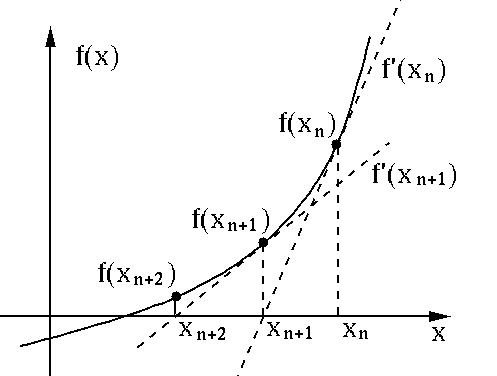
\includegraphics[width=0.8\textwidth]{imagenes/newton.png}
	\end{center}
	\caption{Construcción gráfica de la sucesión dada por el método de Newton-Raphson}
	\label{fig:etiq_7}
\end{figure}

Como se puede ver en la Figura \ref{fig:etiq_7} el método de Newton-Raphson comienza con un valor $x_0$ que es una primera aproximación, y para calcular el siguiente valor de la sucesión toma la pendiente de la función en el punto $(x_0, f(x_0))$, entonces $x_1$ será la intersección del eje de abscisas con la recta tangente que acabamos de ver.
${ }$\\

El algoritmo a seguir es el siguiente:

\begin{itemize}
	\item Paso 0 : Tomar un $x_0$ inicial.
	\item Paso 1 : $x_{n+1} = x_n - \frac{f(x_n)}{f'(x_n)}$.
\end{itemize}

Se puede observar que no siempre es posible calcular el siguiente $x_n$ ya que la derivada de la función en $x_{n-1}$ podría ser $0$.
${ }$\\
${ }$\\

${ }$\\
$\textbf{Regula-Falsi}$
${ }$\\

El algoritmo de Regula-Falsi es un refinamiento de el método de bisección. Al igual que en el método de bisección partimos de un intervalo inicial $[a_0, b_0]$, teniendo $f(a_0)$ y $f(b_0)$ signos opuestos, ya que como dice el Teorema\ref{teo:bolzano} esto nos garantiza que hay una solución dentro de ese intervalo, aunque por el procedimiento que sigue este algoritmo es posible no encontrar soluciones que correspondan con un mínimo o un máximo de la función. Este método va calculando intervalos cada vez mas pequeños que incluyen a la solución.
${ }$\\

Como se puede ver en la Figura \ref{fig:etiq_8}, gráficamente el procedimiento toma la recta que pasa por los puntos $(a_0, f(a_0))$ y $(b_0, f(b_0))$ y toma el punto de intersección de esta con el eje de abscisas el nuevo intervalo se ajustará dependiendo de que el valor de la función en este nuevo punto sea negativo a positivo, $f(a_1) \cdot f(b_1) < 0$.

\begin{teorema}\label{teo:bolzano}
	$\textbf{(de los ceros de Bolzano)}$ Sea una función continua $f : [a,b] \to \mathbb{R}$ tal que $f(a) \cdot f(b) < 0$, entonces existe al menos un $s \in (a,b)$ tal que $f(s) = 0$.
\end{teorema}



El algoritmo de Regula-Falsi es el siguiente:

\begin{itemize}
	\item Paso 0 : Tomar un $a_0$ y $b_0$ iniciales.
	\item Paso 1 : $m_n = \frac{a_n f(b_n) - b_n f(a_n)}{f(b_n) - f(a_n)}$
	\begin{itemize}
		\item Si $f(m_n)=0$, hemos terminado.
		\item Si $f(a_n) \cdot f(m_n) < 0$, $b_n = m_n$.
		\item Si $f(b_n) \cdot f(m_n) < 0$, $a_n = m_n$.
	\end{itemize}
\end{itemize}

\begin{figure}
	\begin{center}
		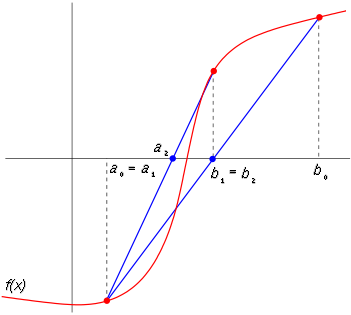
\includegraphics[width=0.8\textwidth]{imagenes/regulaF.png}
	\end{center}
	\caption{Construcción gráfica del método de Regula-Falsi}
	\label{fig:etiq_8}
\end{figure}




${ }$\\
$\textbf{Comparación de métodos}$
${ }$\\


\begin{definicion}
	Sea $p \in \mathbb{R}$ y $p > 1$. Diremos que la sucesión $\{ x^{(k)} \}^{\infty}_{k=1}$ convergente a $s$ de números reales \underline{\textbf{converge}} a $s$ \underline{\textbf{con al menos orden de convergencia $p$}} si $|x^{(k)} -s| \leq \epsilon_k$, $\forall k = 1,2,3...$, siendo $\{ \epsilon_k \}^{\infty}_{k=1}$ una sucesión de números reales positivos tal que
	\[
		\lim_{k \to \infty} \frac{\epsilon_{k+1}}{\epsilon^{p}_{k}} = C
	\]
	con $C > 0$ si $p > 1$, y $0 < C < 1$ si $p = 1$.
	${ }$\\
	
	Por otro lado, si $\epsilon_k = |x^{(k)} -s|$, $\forall k = 1,2,3...$, entonces diremos que la sucesión converge a s con orden de convergencia $p$ y constante asintótica del error igual a $C$.
	\begin{itemize}
		\item Si $p=1$,llamamos lineal al orden de convergencia.
		\item Si $p=2$, la llamamos cuadrática.
	\end{itemize}
\end{definicion}

Hay que tener en cuenta que para mayores valores de $p$ mayor es la rapidez con que converge.
${ }$\\

Para el caso de Newton-Raphson encontramos dos resultados que nos indican cuales son los ordenes de convergencia que nos podemos encontrar a la hora de aplicar ese método. Uno de ellos es para una función cuyo cero queremos encontrar es simple, es decir, $f'(s) \neq 0$ para $s$ raíz de $f$; y el otro para el caso de que la raíz sea un cero múltiple.

\begin{definicion}
	Sea $f \in C^M([a,b])$ y $s$ valor donde $f$ se hace cero, diremos que es de multiplicidad $M$ si y sólo si $f^{(k)}(s) = 0$, $k = 0, ..., M-1$ y $f^{(M)}(s) \neq 0$. Si $M = 1$ se llama cero simple.
\end{definicion}

\begin{teorema}
	Sea $f \in C^2(U_S)$ con $U_S$ un entorno de $s$ tal que $f(s) = 0$ y $f'(s) \neq 0$. Entonces, $\exists \epsilon > 0$ tal que si $|x^{(0)} - s| \leq \epsilon$ la sucesión generada por el método de Newton-Raphson converge a $s$ con convergencia cuadrática y constante asintótica del error $\frac{|f''(s)|}{2|f'(s)|}$.
\end{teorema}

\begin{proof}
	${ }$\\
	
	En lo que sigue consideraremos el desarrollo en serie de Taylor
	\[
		f(x) = f(x_n) + (x - x_n)f'(x_n) + \frac{(x - x_n)^2}{2} f''(\xi)
	\]
	siendo $\xi$ un punto intermedio entre $x$ y $x_n$. Si $x=s$, $s$ una raíz de $f$ y dividiendo por $f'(x_n)$, obtenemos
	\[
		s = x_n - \frac{f(x_n)}{f'(x_n)} - \frac{(s - x_n)^2}{2} \cdot \frac{f''(\xi_n)}{f'(x_n)}
	\]
	siendo $\xi_n$ un punto intermedio entre $s$ y $x_n$. Finalmente usando la expresión del método de Newton-Raphson, tenemos
	\[
		s - x_{n+1} = - (s - x_n)^2 \cdot \frac{2f''(\xi_n)}{f'(x_n)}
	\]
	
	Como $f'(s) \neq 0$ y $f'$ es continua en $U_S$, entonces $\exists \delta > 0$ tal que $f'(x) \neq 0$ $\forall x \in I_{\delta} = [s - \delta, s + \delta]$. Ahora consideremos
	\[
		M = M(\delta) = \frac{\max_{x \in I_{\delta}} |f''(x)|}{2 \min_{x \in I_{\delta}} |f'(x)|}.
	\]

	Por tanto, podemos llegar a que
	\[_
		|s - x_1| \leq M |s - x_0|^2
	\]
	\[_
		M|s - x_1| \leq (M |s - x_0|)^2
	\]
	de donde podemos fácilmente deducir por inducción que
	\[
		|s - x_n| \leq \frac{1}{M} (M |s - x_0|)^{2^n}
	\]
	
	Para terminar de probar la convergencia comprobaremos que existe un $\epsilon > 0$ con $\epsilon < \delta$ tal que $\epsilon M(\epsilon) < 1$. Así que veamos que siempre es posible encontrar dicho $\epsilon$.
	
	\begin{itemize}
		\item Si $\delta M(\delta) < 1$, entonces $\epsilon = \delta$.
		\item Si $\delta M(\delta) \geq 1$, entonces $\epsilon = \delta_1$ donde $0 < \delta_1 < \delta$ y $\delta_1 M(\delta_1) < 1$. Esto posible ya que si
		
		\[
			\delta_1 < \delta \Rightarrow I_{\delta_1} \subset I_{\delta} \Rightarrow
		\]
		\[
			\max_{x \in I_{\delta_1}} |f''(x)| \leq \max_{x \in I_{\delta}} |f''(x)| \;\;\;\; y \;\;\;\; \min_{x \in I_{\delta_1}}|f'(x)| \geq \min_{x \in I_{\delta}}|f'(x)|
		\]
		\[
			\Rightarrow M(\delta_1) \leq M(\delta)
		\]
	\end{itemize}
	
	Por tanto podemos encontrar un $\delta$ tal que $\delta M(\delta) < 1$, es decir, ya que $x_0 \in I_{\delta}$, tenemos $M(\delta)|s - x_0| < 1$. Entonces,
	\[
		|s - x_n| \leq \frac{1}{M} (M |s - x_0|)^{2^n}
	\]
	nos dice que $x_n$ converge a $s$.
	
	Dicho esto, como $\xi_n$ se encuentra entre $s$ y $x_n$ entonces $\xi_n$ tiende a $s$ cuando $n$ tiende a $\infty$. Y por tanto,
	\[
		\lim_{n \rightarrow \infty} \frac{|s - x_{n+1}|}{|s - x_{n}|^2} = - \lim_{n \rightarrow \infty} \frac{f''(\xi_n)}{2f'(x_n)} = - \frac{f''(s)}{2f'(s)}.
	\]
\end{proof}

\begin{teorema}
	Sea $f \in C^2(U_S)$ con $U_S$ un entorno de $s$ tal que $f(s) = 0$. Entonces, el método de Regula-Falsi converge a $s$ con orden de convergencia lineal y constante asintótica del error $(\frac{|f''(s)|}{2|f'(s)|})^{(\varphi - 1)}$.
	
\end{teorema}

\begin{proof}
	Para cada iteración $n$ de Regula-Falsi calculamos la ecuación de la recta que pasa por los puntos $(a_n, f(a_n))$ y $(b_n, f(b_n))$
	\[
		y - f(b_n) = \frac{f(b_n) - f(a_n)}{b_n - a_n}(x - b_n),
	\]
	ahora haciendo $y = 0$ obtenemos la fórmula vista para el algoritmo
	\[
		m_n = b_n - f(b_n) \frac{b_n - a_n}{f(b_n) - f(a_n)} = \frac{a_n f(b_n) - b_n f(a_n)}{f(b_n) - f(a_n)}
	\]
	
	Vamos a representar el error en la n-ésima iteración por $e_n = m_n - s$ y para demostrar que la convergencia es lineal usaremos la siguiente expresión obtenida de restar $s$ a la expresión anterior
	\[
		m_n - s = b_n - s - f(b_n) \frac{b_n - a_n}{f(b_n) - f(a_n)}
	\]
	
	También haremos uso del desarrollo en serie de Taylor para aproximar la función $f$
	\[
		f(x) = f(s) + (x - s) f'(s) + \frac{(x - s)^2}{2} f''(s)
	\]
	donde sabemos que $f(s) = 0$ y por tanto para $a_n$, $b_n$
	\[
		f(a_n) = (a_n - s) f'(s) + \frac{(a_n - s)^2}{2} f''(s)
	\]
	\[
		f(b_n) = (b_n - s) f'(s) + \frac{(b_n - s)^2}{2} f''(s).
	\]
	Calculamos
	\[
		f(b_n) - f(a_n) = f'(s) (b_n - a_n) + \frac{f''(s)}{2}[(b_n - s)^2 - (a_n - s)^2]
	\]
	\[
		= (b_n - a_n) [f'(s) + \frac{f''(s)}{2} (b_n + a_n - 2p)],
	\]
	con esto y $f(b_n)$ podemos obtener
	\[
		m_n - s = (b_n - p)[1 - \frac{f'(s) + \frac{f''(s)}{2} (b_n - s)}{f'(s) + \frac{f''(s)}{2} (b_n + a_n - 2p)}]
	\]
	\[
		= (b_n - p) (a_n - p) \frac{f''(s)}{2 f'(s) + f''(s) (b_n + a_n - 2p)}
	\]
	
	Tengamos en consideración que llega un momento en el que el intervalo es tan pequeño que el signo de su derivada y segunda derivada se conserva, supongamos que esto ocurre en una iteración $i$. Entonces, sin perdida de generalidad supondremos que $f'(x) \geq 0$ y $f''(x) \geq 0$ para $x \in [a_i, b_i]$. Llegados a este punto, por la forma que toma la función habrá un extremo del intervalo que quedará fijo para $n \geq i$. A partir de esto y considerando que $e_{n-1} = m_{n-1} - s = b_n - s$
	
	\[
		e_n = e_{n-1} (a_n - s) \frac{f''(s)}{2 f'(s) + f''(s) (e_{n-1} + a_n - p)}
	\]
	
	Definiendo
	\[
		\lambda \simeq \frac{l f''(s)}{2 f'(s) l f''(s)},
	\]
	donde $l = (a_n - s)$ cuando $a_n$ queda fijo y $l = (b_n - s)$ cuando $b_n$ queda fijo, podemos concluir que
	\[
		e_n \simeq \lambda e_{n-1}
	\]
	
	Por tanto la sucesión de Regula-Falsi converge con orden de convergencia lineal.
\end{proof}


${ }$\\
$\textbf{Criterio de parada}$
${ }$\\

El algoritmo que queremos implementar va calculando los elementos de una sucesión que converge a la solución pero en la mayoría de los casos no llega a ser la solución exacta y hay infinitos términos de la sucesión por lo que tenemos que elegir un método que nos diga cuando queremos que pare de calcular elementos de la sucesión. Usaremos como método uno de los siguientes criterios de parada: para cuando se hayan realizado un número determinado de iteraciones, parar cuando $|f(x_n)| < \epsilon$, parar cuando $|x_{n-1} -x_n| < \epsilon$ donde $\epsilon > 0$. En este caso vamos a usar que $|f(x_n)| < \epsilon$.


${ }$\\
$\textbf{INTRODUCCIÓN}$
${ }$\\

Las ecuaciones implícitas de superficies son de la forma $F(x, y, z) = 0$ esta forma es adecuada para imágenes con sombreado. Las coordenadas de pixeles son sustituidas por $x$ e $y$ y la ecuación es resuelta para z. Los algoritmos para dibujar tales objetos se han desarrollado principalmente para funciones polinomiales de primer y segundo orden, una subcategoría conocida como superficies algebraicas. Este artículo presenta un nuevo algoritmo aplicable a otras formas funcionales, en particular a la suma de varias distribuciones de densidad gaussianas. El algoritmo fue creado para modelar mapas de densidad electrónica de estructuras moleculares, pero puede ser utilizado para otras formas artísticamente interesantes.

La tecnología de crear imágenes realistas y visualmente interesantes de tres
las formas dimensionales están avanzando en muchos frentes. Uno de ellos es el desarrollo de algoritmos para dibujar superficies curvas directamente desde sus definiciones matemáticas en lugar de dividirlas en grandes cantidades de polígonos. Dos clases de superficies que han recibido atención son las superficies paramétricas cuádruples y las bivariadas. Las superficies paramétricas bivariadas se generan mediante tres funciones de dos variables (la mayoría de las veces son polinomios), ya que las variables adquieren diferentes valores.

Superficies cuádricas, por otro lado, son soluciones de ecuaciones de segundo orden.

\[
	ax^2 + bxy + cxz +dx +ey^2 +fyz +gy + hz^2 + iz +j = 0.
\]

Esta clase de superficies incluye formas tales como esferas, conos o hiperboloides de revolución. Como podemos ver las cuadricas son soluciones de ecuaciones implicitas que como hemos dicho son de la forma $F(x, y, z) = 0$.

Este documento examina una solución más general al problema de imágenes para tales superficies y describe en detalle su aplicación a una clase de superficies que están estrechamente relacionadas con los cuadrículas pero que tienen una gama más amplia de formas.


${ }$\\
$\textbf{EL MODELO}$
${ }$\\

El problema que motivó este documento es el familiar en los gráficos por computadora de mostrar modelos moleculares. Esto se hace con mayor frecuencia con un modelo de bola y bastón o un modelo de esfera llenadora de espacio. En cualquier caso, el modelo consiste en una colección posiblemente interseccionada de dos formas básicas: esferas y cilindros. Para dibujar una imagen del modelo, las esferas y los cilindros se pueden dividir fácilmente en polígonos y pasar a un algoritmo convencional de representación de polígonos. Alternativamente, se puede emplear cualquiera de varios algoritmos de superficie curva, y, de hecho, se han formulado varios algoritmos de propósito especial [6, 8, 9] para manejar eficientemente solo estas dos formas para la visualización rápida de estructuras moleculares grandes.

En interés tanto de la variedad artística como de la precisión científica, se buscó un nuevo modelo que se separe del molde de bola y adhesivo / relleno de espacio. Se deseaba hacer que los enlaces entre los átomos se parecieran más a los que se muestran en la Figura 1. Esto es, de hecho, más parecido a lo que podría parecer una nube de densidad de electrones real para un enlace covalente. Además, a los efectos de la animación, este vínculo debe estirarse y contraerse de una manera agradable, ya que vibra, rompiendo a medida que un átomo se aleja por completo de la molécula. Esto se ilustra en la Figura 2.

Un enfoque convencional podría ser modelar dicha forma a través de las superficies bicúbicas o cuádricas ya familiares. Esto es moderadamente factible para un enlace aislado pero se vuelve difícil para moléculas más elaboradas con varios enlaces superpuestos (por ejemplo, estructuras de anillo). Además, los cambios topológicos que deben ocurrir cuando se rompe un enlace son difíciles de manejar de manera automatizada. Por estas razones, se utilizó un modelo matemático básico que es similar en forma a una simulación real de mapas de densidad de electrones. La mecánica cuántica representa el electrón en un átomo como una función de densidad de la ubicación espacial. Una función de muestra para un átomo de hidrógeno es

\[
	D(x, y, z) = exp(-ar)
\]
donde $r = \sqrt{(x-x_1)^2 + (y-y_1)^2 + (z-z_1)^2}$ y $(x_1, y_1, z_1)$ la localización del átomo.

Podemos representar esta función para una colección de átomos sumando la contribución de cada átomo por separado.
\[
	D(x, y, z) = \sum_{i} b_i exp(-a_i r_i)
\]
donde $r_i$ es la distancia de $(x,y,z)$ al centro del átomo $i$.

Una superficie se puede definir como aquellos puntos donde esta función de densidad es igual a una cantidad umbral:
\[
	F ( x, y, z) = D ( x, y, z) - T.
\]

Tenga en cuenta que todos los puntos dentro de la superficie tienen densidades de electrones mayores que T. A los efectos de la eficiencia computacional, la función realmente implementada fue de forma similar:
\[
	D(x, y, z) = \sum_{i} b_i exp(-a_i r^{2}_{i})
\]
Esto no requiere tomar una raíz cuadrada. El término exponencial es simple
Golpe gaussiano centrado en ri, con altura bi y desviación estándar ai. Ajustando los parámetros ai y bi, se pueden lograr diferentes efectos para la misma disposición de átomos. Estos efectos alteran el "blobbiness" del objeto. De hecho, para fines de modelado, es más útil para un diseñador especificar estos dos parámetros en términos del radio del átomo en aislamiento y un parámetro de blobbiness. El radio de un átomo aislado Ri se encuentra al establecer
\[
	T = b_i exp(-a_i R^{2}_{i}) = exp (-a_i R^{2}_{i} + ln (b_i))
\]
entonces el ai puede ser elegido para ser
\[
	a_i = - \frac{ln(T/b_i)}{R^{2}_{i}}
\]
Podemos definir el parámetro blobbiness para ser
\[
	B_i = ln(T/b_i)
\]
de modo que (resolviendo para bi)
\[
	b_i = T exp(-B_i)
\]
La contribución de densidad neta de un átomo en términos de los dos parámetros que definen la forma Ri y Bi es
\[
	D_i(x,y,z) = T \; exp ( \frac{B_i}{R^{2}_{i}}r^{2}_{i} -B_i)
\]
Tenga en cuenta que Bi debe ser negativo para garantizar que la función de densidad vaya a cero a medida que ri va al infinito.

Como hay un factor de T en cada átomo contribuyente, el valor del umbral ahora es irrelevante; podemos establecerlo en algún valor canónico como 1. Uno puede obtener el mismo efecto que cambiar el umbral ajustando los factores de escala, bi, de los términos individuales (es decir, ajustando los parámetros de blobbiness Bi). Sin embargo, para mayor claridad, generalmente escribimos el umbral como T, en el entendimiento de que T = 1. Un valor de umbral canónico de 1 es particularmente conveniente ya que su logaritmo es 0. La superficie definida por un átomo aislado, definida por el ajuste Di = T, es entonces una superficie cuádrica convencional. Esto se ve tomando el logaritmo de ambos lados de la ecuación anterior, produciendo 0 = (Bi / R2i) r2i - Bi. En la Figura 3 se muestra una imagen de muestra que muestra un rango de tales parámetros.

${ }$\\
$\textbf{EL ALGORITMO DE RENDERIZADO}$
${ }$\\

Las superficies definidas algebraicamente son intrínsecamente adecuadas para los algoritmos de conversión de trama. La estructura general de dicho algoritmo es sencilla: para cada ubicación de píxeles (xs, ys) la ecuación algebraica de definición se reduce a una ecuación univariante en z. Las soluciones a esta ecuación (si las hay) producen la profundidad z de la superficie en ese píxel. En el caso de las superficies cuádricas más comunes, esta solución es fácil de obtener. En el caso de las superficies más generales que se describen aquí, la solución debe obtenerse numéricamente. La parte importante del algoritmo descrito aquí es una técnica para acelerar este cálculo.

${ }$\\
$\textbf{Algoritmo básico}$
${ }$\\

Para un píxel particular, el cuadrado de la distancia desde el centro del átomo i, Pi, a un punto en el rayo de visión, $z \overline{R}$, se reduce a un polinomio cuadrático en z.
\[
	r^{2}_{i} = (z\overline{R} - \overline{P}_i)\cdot(z\overline{R} - \overline{P}_i) = z^2(\overline{R} \cdot \overline{R}) - 2 z (\overline{R} \cdot \overline{P}_i) + (\overline{P}_i \cdot \overline{P}_i)
\]
Esta expresión es algebraicamente correcta, pero desafortunadamente es susceptible de un error de redondeo. La razón para esto se puede ver en la Figura 4.

La función puede ser una parábola bastante estrecha centrada posiblemente bastante atrás en el eje z. Si bien los valores comúnmente encontrados para los coeficientes de esta ecuación no presentan por sí mismos problemas, la solución de la ecuación requiere tomar diferencias de sus productos. Esto puede exceder fácilmente la precisión de la aritmética de precisión simple. Para evitar la necesidad de una aritmética de precisión múltiple, adoptamos una representación más geométricamente significativa
\[
	r^{2}_{i} = (\overline{R} \cdot \overline{R})(z - z^{2}_{mi}) + M_i
\]
donde
\[
	z_{mi} = (\overline{R} \cdot \overline{P}_i)/(\overline{R} \cdot \overline{R}) \;\;\;\;\;\; y \;\;\;\;\;\; M_i = (z_{mi} \overline{R} - \overline{P}_i) \cdot (z_{mi} \overline{R} - \overline{P}_i)
\]
Aquí, zmi es la distancia z del mínimo local, Mi, de ri. Cada término en la función de densidad es, por lo tanto, una función de bache gaussiana de z centrada en zmi ,. La función total es la suma de varios de estos golpes. El valor de profundidad z visible es la primera ubicación donde esta función excede el valor T. Esto se muestra en la Figura 5.

Si solo se ve un átomo, la profundidad z se puede encontrar analíticamente estableciendo el término de densidad para ese átomo igual al valor umbral de 1.
\[
	T = 1 = exp ( -a_i r^{2}_{i} - B_i)
\]
Tomando el logaritmo de ambos lados y sustituyendo nuestra fórmula por r2i,
\[
	0 = a_i [(\overline{R} \cdot \overline{R})(z-z^{2}_{mi}) + M_i] + B_i.
\]
Resolviendo z (nótese que la raíz cuadrada negativa se toma para obtener la solución más cercana al ojo),
\[
	z = z_{im} - \sqrt{\frac{a_i M_i + B_i}{-a_i (\overline{R} \cdot \overline{R})}}.
\]

${ }$\\
$\textbf{Solución iterativa}$
${ }$\\

Si hay más de un átomo, una solución analítica no es factible y debemos recurrir a métodos numéricos. Dos métodos populares para la solución iterativa de tales ecuaciones son Newton iteration y "regula falsi".

La iteración de Newton funciona comenzando con una suposición inicial y refinándola al aproximar la función D con una línea recta tangente a la función en ese punto. La solución de esta ecuación lineal produce una nueva suposición, $z_new$.
\[
	z_{new} = z - \frac{D(z) - T}{D'(z)}
\]
Los derivados se obtienen fácilmente a partir de la forma funcional.
\[
	\frac{dD}{dz} = D' = \sum_{i} -2 a_i (\overline{R} \cdot \overline{R}) (z - z_{mi}) exp(-a_i r^{2}_{i} - B_i)
\]
Tenga en cuenta que este cálculo utiliza muchos cálculos en común con el cálculo de D, por lo que la evaluación de D y D 'es relativamente económica.

Regula falsi comienza con dos conjeturas iniciales que se sabe que entre corchetes la solución: Zn, donde D (zn) <T, y zf, donde D (zf)> T. Genera una nueva suposición dibujando una línea entre (z ,, D (zn)) y (zf, D (zf)) y resolver para T.
\[
	z_{new} = \frac{z_n (D(z_f) - T) - z_f ( D(z_n) - T)}{D(z_f) - D(z_n)}
\]
El valor real de $D (z_new)$ se calcula. Si $D (z_new) <T$ entonces $z_new$ reemplaza a zn. De lo contrario, reemplaza zf. Por lo tanto, el rango entre zn y zf se contrae continuamente alrededor de la solución correcta.

Si la conjetura inicial es lo suficientemente cercana a la solución real, la iteración de Newton converge rápidamente. Si no está cerca, sin embargo, divergerá. Se garantiza que Regula falsi converge pero lo hace más lentamente. Por lo tanto, hemos adoptado una solución híbrida. Un valor para $z_new$ se calcula mediante la iteración de Newton. Si este valor está fuera del rango (Zn, Zf), entonces el valor se vuelve a calcular a partir de la fórmula regula falsi. Este proceso se repite hasta que el valor de $| D (z_new) - T |$ es menor que alguna tolerancia de error t.

Para generar el primer rango inicial de suposiciones, dependemos de algunas heurísticas basadas en nuestro conocimiento de la forma funcional. Esperamos que la solución esté en o cerca de las soluciones a las protuberancias atómicas individuales (Figura 6) o al máximo local de una protuberancia si no supera el valor umbral T (Figura 7).

Por lo tanto, hacemos una lista de posibles valores iniciales de estimación z y los ordenamos en orden ascendente de z. La lista ordenada se escanea de adelante hacia atrás y, para cada elemento, se calcula el valor real de la función (es decir, la suma de todas las contribuciones de átomos). Si esto es menor que el valor umbral, se supone que el máximo local de D cerca de aquí no alcanza el umbral y se evalúa el siguiente elemento de la lista. Si excede el valor umbral, esa z se usa como el valor inicial de zf y el elemento de la lista anterior se usa como el valor inicial de zn. Ver la Figura 8.

${ }$\\
$\textbf{Cálculos de intensidad}$
${ }$\\

Cuando se encuentra una solución z, se sustituye en eq. (*) para obtener las ubicaciones xey del punto visible en la superficie en el espacio de visualización. Para calcular una intensidad, es necesario encontrar la superficie normal en este punto. Esto se puede encontrar tomando el gradiente de la función de definición de superficie, F.
\[
	N = \left[ {\begin{array}{ccc}
		\frac{\partial F}{\partial x}, & \frac{\partial F}{\partial y}, & \frac{\partial F}{\partial z} \\
		\end{array} } \right]
\]
Para la función que estamos usando aquí, esto se hace fácilmente. Por ejemplo, el componente x será
\[
	\frac{dF}{dx} = D' = \sum_{i} -2 a_i (x - x_i) exp(-a_i r^{2}_{i} - B_i)
\]
Finalmente, podemos permitir que las propiedades reflectantes de la superficie (como el color) varíen sobre la superficie mezclándolas de acuerdo con las contribuciones de cada átomo. Esto se hace tomando una suma ponderada de la propiedad superficial de cada átomo, el peso elegido como el valor de Di de ese átomo. (Recuerde que estas suman el valor umbral de 1.0.) Alternativamente, como en la facilidad de los diagramas que se muestran aquí, podemos encontrar el átomo con el valor más alto de Di en el punto visible y usar sus propiedades de superficie.

${ }$\\
$\textbf{Optimizando el algoritmo}$
${ }$\\

Para las imágenes que contienen más de unos pocos átomos (hasta 4000 en algunas de las imágenes requeridas para este proyecto), la suma de la función D sobre todos los átomos está computacionalmente fuera de la cuestión. Afortunadamente, para cualquier píxel dado, la mayoría de los átomos están lo suficientemente lejos del rayo de escaneo, por lo que su contribución a la función D es insignificante. Por lo tanto, podemos economizar considerablemente utilizando en los cálculos solo los átomos que están "cerca" del rayo de exploración. El término "cerca" tiene un significado preciso al encerrar cada átomo en una esfera definida por
\[
	D_i (x,y,z) = tT,
\]
donde el valor t es la misma tolerancia de error utilizada como criterio de convergencia. Si el rayo de escaneo se cruza con esta esfera, debe haber puntos a lo largo de ella donde la contribución a D sea lo suficientemente grande como para importar. Si, por otro lado, el rayo escaneado está separado de la esfera circundante, entonces todos los puntos en él contribuyen menos que el error introducido por las condiciones de terminación de la solución numérica. El átomo puede omitirse.

El valor de la tolerancia al error, por supuesto, determina la calidad de la imagen. Una tolerancia mayor será más rápida pero la imagen tendrá un poco de ruido agregado. La Figura 9 muestra los resultados obtenidos con diferentes valores de t. El halo alrededor de cada ejemplo indica los píxeles cubiertos por las esferas de los átomos. Los errores en la superficie comienzan a ser aparentes con t = 0.03. Aparecen inicialmente como un pliegue a través del resalte en la parte superior de la forma.

El proceso de mantener una lista de átomos "cercanos" durante la renderización es similar al de mantener una lista de polígonos potencialmente visibles en algoritmos de representación de polígonos más convencionales (o quizás, de manera más adecuada, mantener una lista de esferas visibles en un dibujo de esferas) programa).

Comenzamos con el bucle externo (y). Para inicializar el ciclo, las esferas circundantes de todos los átomos se proyectan en el espacio de la pantalla y se calculan los valores y máximos y mínimos visibles. Las matemáticas exactas para esto se dan en la siguiente sección. La lista de átomos se ordena en mínimo y, formando la lista "y-enter". Durante el ciclo de exploración y, mantenemos una lista adicional de "y activados" de todos los átomos cuya esfera envolvente incluye el plano de exploración actual. Las adiciones y eliminaciones de esta lista se realizan de forma incremental cada vez a través del ciclo. Es decir, cada vez que $y_s$ se incrementa, se examina el elemento superior en la lista y-enter. Si ahora está por encima de los nuevos $y_s$, se mueve a la lista y-active y se examina el siguiente elemento en la lista y-enter. Cuando la parte superior de la lista y-enter está debajo de los nuevos $y_s$, sabemos que todos los átomos que ingresaron se han agregado. Ahora examine la lista activa para las eliminaciones. El $y_min$ de cada átomo en la lista y-active se prueba contra los nuevos $y_s$, y si está por encima de él, el elemento se elimina. Ver la Figura 10.

Dentro del bucle $ y $ hay un bucle $ x $ que recorre la pantalla. Aquí mantenemos una lista x-active con los candidatos provenientes de la lista y-active. Esto se hace de una manera exactamente análoga al ciclo y. Para cada elemento en la lista y-active, la esfera circundante se proyecta en la pantalla y se calcula el valor x máximo y mínimo. La lista y-active se ordena en $x_ {min}$ y se convierte en la lista x-enter. Dado que la lista y-active es de hecho idéntica a la lista x-enter, siempre se mantiene ordenada en x, desde la línea de exploración hasta la línea de exploración. Todas las adiciones se combinan en la lista utilizando un tipo de intercambio. A medida que el escaneo avanza de izquierda a derecha, se examina la lista x-enter para ingresar átomos y agregarlos a la lista x-active. La lista x-active se analiza en busca de átomos que salen. Vea la Figura 11.

En este punto tenemos, para un píxel dado, una lista de todos los átomos cuya esfera circundante intersecta el rayo de escaneo actual a través de ese píxel. Esta lista representa un sacrificio significativo de la totalidad de los átomos a solo aquellos que son relevantes para el píxel actual. Sin embargo, hay un nivel más de sacrificio disponible. Esto está en la dirección z. En la Sección 3.3 describimos la técnica para encontrar un punto inicial para la solución iterativa como un escaneo de adelante hacia atrás a través de una lista ordenada en z de posibles puntos de solución. Si, antes de este zscan, calculamos los valores Zmin / Zmax de las intersecciones de las esferas circundantes con el rayo escaneado, podemos mantener una lista z-active a medida que progresa zscan. En este caso, los valores de z examinados para las pruebas de entrada / salida no son valores enteros equiespaciados como en los casos xey. En su lugar, se toman uno a la vez de la lista z potencial. Sin embargo, esto no altera el principio básico. Ver la Figura 12.

Cuando ejecutamos el ciclo de iteración, la suma del Di se tomará solo para aquellos átomos lo suficientemente cercanos a la conjetura inicial como para importar. Por ejemplo, para la imagen que contiene más de 4000 átomos (Figura 13), había como máximo 6 átomos en la lista z-activa para la iteración y usualmente mucho menos.


${ }$\\
$\textbf{Cálculo del rango en x, y, z}$
${ }$\\

En esta sección, indicamos explícitamente cómo calcular las extensiones x, y y z de la esfera circundante de un átomo. Tales esferas adjuntas están definidas, como se describe en la Sección 3.5, por la ecuación
\[
	tT = D_i = exp (-a_i r^{2}_{i} - B_i)
\]
Tomando el logaritmo (y recordando que T = 1), transformamos esto en la ecuación para una superficie cuádrica
\[
	0 = a_i r^{2}_{i} + (B_i + ln(t))
\]
Para calcular $z_ {min} / z_ {max}$ para la prueba de rango de zscan, sustituimos la expresión por r2i en términos de z:
\[
	0 = a_i [(\overline{R} \cdot \overline{R})(z-z_{mi})^2 + M_i] + (B_i + ln(t))
\]
y resolviendo para z:
\[
	z_{min} = z_{mi} - D_z \;\;\;\;\;\;\; y \;\;\;\;\;\;\; z_{min} = z_{mi} - D_z
\]
donde
\[
	D_z = \sqrt{\frac{a_i M_i + B_i + ln(t)}{-a_i(\overline{R} \cdot \overline{R})}}
\]
Habrá dos raíces en esto siempre que la expresión bajo el radical sea positiva. La curva definida al establecer esto igual a cero definirá la proyección de los contornos de la silueta de la esfera circundante en la pantalla:
\[
	a_i M_i + B_i + ln(t) = 0
\]
Sustituyendo la definición de Mi y $z_ {mi}$ podemos transformar esto en
\[
	\Delta (\overline{R} \cdot \overline{R}) - (\overline{R} \cdot \overline{P}_i)^2 = 0
\]
donde $\Delta = (\overline{P}_i \cdot \overline{P}_i) + \frac{B_i + ln(t)}{a_i}$.

Recordando que $R = (x_z, y_z, 1)$ obtenemos

\[
	\Delta (x^{2}_{z} + y^{2}_{z} + 1) - (x_z x_i + y_z y_i + z_i)^2 = 0.
\]

Ahora para una línea de escaneo particular, $y_z$ es constante. Luego tenemos una ecuación cuadrática en $x_z$ cuyas soluciones dan el rango en $x_z$ para esa línea de escaneo.
\[
	x^{2}_{z} (\Delta - x^{2}_{i}) + x_z (-2 x_i (y_z y_i + z_i)) + (\Delta (y^{2}_{z} + 1) - (y_z y_i + z_i)^2) = 0.
\]
Las soluciones a esta ecuación $(x_ {z \; min}, x_ {z \; max})$ aún se deben convertir a coordenadas de píxel $(x_ {s \; min}, x_ {s \; max})$ por referencia a eq . (*)

La ecuación anterior tendrá dos raíces en todos los valores de $ y_z $ para los cuales su discriminante es positivo. Los valores de $ y_z $ para los que este discriminante se convierte en cero, por lo tanto, arrojan el máximo y mínimo $ y_z $ para los cuales la esfera que los contiene es visible.
\[
	4 x^{2}_{i}(y_z y_i + z_i)^2 - 4(\Delta - x^{2}_{i})(\Delta (y^{2}_{z} +1) - (y_z y_i + z_i)^2 ) = 0.
\]
De nuevo, las dos soluciones para $ y_z $ de esta ecuación se deben convertir a coordenadas de píxeles mediante eq. (*)

En los casos x e y, el rango de píxeles para la esfera circundante debe intersecarse con el rango de píxeles de la pantalla. Esto significa que estamos realizando un recorte en el espacio de la pantalla. Si el rango de la esfera está completamente fuera de la pantalla, puede eliminarse por completo.

${ }$\\
$\textbf{Sincronización}$
${ }$\\

El algoritmo de renderizado, al hacer algunas formas bastante interesantes, no es terriblemente rápido. En un esfuerzo por ver dónde se gasta el tiempo dentro del algoritmo, fue instrumentado para medir el tiempo. La Tabla 1 muestra los resultados para los cálculos implicados en la generación de la Figura 14, que contiene 64 átomos. Nuevamente, el halo alrededor de la molécula representa las esferas de los átomos e indica el rango de píxeles sobre el que se realizan los cálculos.

Tenga en cuenta que aunque las rutinas $y_ {scan}$ y $x_ {scan}$ tardan bastante tiempo (ya que tienen que ocuparse de listas activas más grandes), su contribución neta al tiempo de ejecución es pequeña ya que solo se llaman una vez por imagen y una vez por línea de exploración potencialmente ocupada, respectivamente. La rutina z calc es donde se calculan los valores de $z_ {mi}$, $M_i$, etc., para todos los átomos en la lista z-active. Esto es lo que toma la mayor parte del tiempo. Parte de la razón para esto no es tanto la cantidad de veces interrumpidas en la rutina como la gran cantidad de veces que se llama. Se llama una vez para cada píxel cubierto por cualquier esfera circundante, mientras que la rutina de iteración y sombreado se llama una vez por cada píxel ocupado.

También presentamos histogramas de los tamaños de las listas activas para cada uno de los escaneos anidados. Cada contenedor del histograma cuenta el número de veces que un tamaño determinado de la lista activa se pasa a la rutina. Tenga en cuenta que, debido al proceso de eliminación selectiva, las rutinas de iteración y sombreado generalmente se llamaban con listas activas de longitud 3 o inferior. Ver la Figura 15


${ }$\\
$\textbf{Modelado jerárquico}$
${ }$\\

La implementación de este algoritmo se realizó en un PDP-11, que permite un espacio de direcciones limitado para los programas de usuario. No hay suficiente memoria de usuario para un programa que hace tanto el modelado como la representación para sistemas de átomos del tamaño deseado. En consecuencia, el proceso se divide en dos programas que se comunican a través de un archivo temporal. Este archivo es, de hecho, solo la lista y-enter ordenada en $y_{max}$ para el volumen adjunto de cada átomo. Un programa de modelado de propósito general acepta comandos que controlan los parámetros de posicionamiento y blobbiness de átomos, iluminación global, parámetros de visualización, etc. Luego escribe la lista y-enter en el archivo atemporary. El programa de renderizado luego lee en este archivo, átomo por átomo, a medida que el escaneo avanza por la pantalla. Esto libera el programa de renderizado de cualquier restricción sobre el número total de átomos visibles. Solo necesita leer un átomo antes que él en el archivo y-enter list para poder saber cuándo el próximo átomo ingresará en la lista y-active. Internamente, solo mantiene la lista y activa y, por lo tanto, tiene restricciones solo en la cantidad máxima de átomos visibles en cualquier línea de escaneo. (Esta técnica también ha sido utilizada por el autor en programas de representación de polígonos y programas de representación de parches bicúbicos, las listas en esos casos son de polígonos o parches).

Todavía hay algunos límites en la cantidad máxima de átomos que puede mantener el programa de modelado. Estos se pueden relajar insertando un módulo de clasificación separado entre el modelador y el renderizador. El modelador no necesita poder almacenar todos los átomos en una escena. Simplemente se ocupa de la interpretación de la línea de comandos, el establecimiento de parámetros y la transformación de átomos para visualizar el espacio. Escribe la lista de átomos tal como la lee de un archivo de definición de molécula. El clasificador es un pequeño programa con una gran matriz. Lee el archivo y-enter list, ordena los datos y los vuelve a escribir.

Para los propósitos del modelado de moléculas polimerizadas grandes (como ADN) se empleó un esquema de modelado jerárquico alternativo. Los polímeros están formados por una gran colección de algunos módulos básicos. Para el ADN, estos módulos son los cuatro nucleótidos y unos pocos radicales libres utilizados para simular el proceso de replicación. Cada módulo se modela como un cuerpo rígido en una posición y orientación arbitrarias. La definición de un módulo enumera sus átomos constituyentes y el radio de una esfera circundante para todo el módulo. Cuando se va a crear una imagen, los módulos se ordenan primero en un orden basado en el mínimo $ y_s $ de sus esferas adjuntas. A continuación, se realiza un escaneo en la dirección y para generar la lista completa de y-enter de átomos directamente en orden ordenado. Para cada nuevo valor de $ y_s $, se examina la lista del módulo y para ver si alguno de los módulos se ha activado. Cuando un módulo se activa, se expande en sus átomos constituyentes que luego se transforman en espacio de visualización de acuerdo con la orientación y posición del módulo. Estos átomos se agregan a un conjunto candidato y-enter. Cuando se hayan expandido todos los módulos recientemente activados, se examinará el grupo y-enter pool candidato. Cualquier átomo que haya sido realmente visible en la línea de exploración se escribe en el archivo y-enter. La ventaja de este proceso es que el grupo candidato y-enter nunca llega a ser muy grande y, por lo tanto, puede manejar grandes estructuras.

${ }$\\
$\textbf{Extensiones}$
${ }$\\

El algoritmo inicial fue ideado para una tarea de propósito especial. Examinamos aquí algunas generalizaciones simples del proceso para dar una gama más amplia de formas que se pueden modelar.

${ }$\\
$\textbf{Método 1}$
${ }$\\

Una extensión obvia de las formas definidas hasta ahora es proporcionar formas primitivas no esféricas. Recuerde que la ecuación de definición original consistía en términos

\[
	exp(-a_i r^{2}_{i} - B_i).
\]

El exponente de e es solo un cuadric de caso especial:
\[
	-a_i r^{2}_{i} - B_i = -a_i((x - x_i)^2 + (y - y_i)^2 + (z - z_i)^2) - B_i
\]
\[
	(xyz1)(-a_i)  \left( {\begin{array}{cccc}
		1 & 0 & 0 & -x_i \\
		0 & 1 & 0 & -y_i \\
		0 & 0 & 1 & -z_i \\
		-x_i & -y_i & -z_i & P\\
		\end{array} } \right) \left( {\begin{array}{cccc}
		x \\
		y \\
		z \\
		1 \\
		\end{array} } \right),
\]
donde,
\[
	P = x^{2}_{i} + y^{2}_{i} + z^{2}_{i} + \frac{B_i}{a_i}.
\]

Al permitir cuadrics generales aquí, podemos tener elipsoides, cilindros, planos, etc., como primitivas de modelado. Esto se hace comenzando con una esfera de unidad canónica en el origen definido por
\[
	0 = (xyz1) \left( {\begin{array}{cccc}
		-B_i & 0 & 0 & 0 \\
		0 & -B_i & 0 & 0 \\
		0 & 0 & -B_i & 0 \\
		0 & 0 & 0 & -B_i \\
		\end{array} } \right) \left( {\begin{array}{cccc}
		x \\
		y \\
		z \\
		1 \\
		\end{array} } \right),
\]

Esto se escala, gira y traduce a la ubicación deseada mediante las técnicas de transformación estándar para cuadrículas [1], es decir, multiplicar a la izquierda por el inverso de la matriz de transformación y a la derecha por la transposición de la inversa.

\[
	Q' = T^{-1}QT^{-1t}
\]
donde $T$ es una matriz de transformación tal que $(x' \; y' \; z' \; w) = (x \; y \; z \; w)T$.

Esta expresión se elige para preservar la relación:

\[
	if \; (x\;y\;z\;w)Q(x\;y\;z\;w)^{t} = 0
\]
\[
	then \; (x'\;y'\;z'\;w')Q(x'\;y'\;z'\;w')^{t} = 0
\]

El lector puede verificar que escalando la matriz por $ R_i $ y traduciéndola a $ (x_i, y_i, z_i) $ uno obtiene solo la formulación de caso especial que utilizamos anteriormente para las esferas puras. La generalización de la mayoría de las otras ecuaciones en la discusión anterior se puede realizar haciendo los siguientes reemplazos:
\[
	a_i(\overline{R} \cdot \overline{R}) \;\;\;\;\; \to \;\;\;\;\; \overline{R}Q'\overline{R}^t
\]
\[
	a_i(\overline{P}_i \cdot \overline{R}) \;\;\;\;\; \to \;\;\;\;\; \overline{R}Q'\overline{W}^t
\]
\[
	a_i(\overline{P}_i \cdot \overline{P}_i) \;\;\;\;\; \to \;\;\;\;\; \overline{W}Q'\overline{W}^t
\]
donde
\[
	Q' = \;\; transformed \;\; (4x4) \;\; quadric \;\; matrix
\]
\[
	W = (0\;0\;0\;1)
\]
\[
	W = (x_z\;y_z\;1\;0)
\]
Una imagen de muestra aparece en la Figura 16.

Para formas de extensión infinita, como cilindros, el cálculo de los valores máximo / mínimo en $ x_s $ o $ y_s $ puede producir un rango infinito. Esto ocurre cuando no hay soluciones para el rango que determina las ecuaciones cuadráticas de la Sección 3.6. Para manejar estas situaciones correctamente, debemos recordar que estamos resolviendo estas ecuaciones no tanto para encontrar sus ceros sino para encontrar la región donde el polinomio cuadrático es positivo (ya que su raíz cuadrada es necesaria más adelante). En el caso general, esto puede producir un tramo finito (para elipsoides), un tramo infinito (el eje de un cilindro) o dos tramos semiinfinitos (hiperboloides). Con el cuidado apropiado al examinar el polinomio, estos casos se pueden distinguir fácilmente.

${ }$\\
$\textbf{Método 2 : Volumenes negativos}$
${ }$\\

Otra extensión es permitir valores negativos para $ b_i $. Esto efectivamente da volúmenes negativos. No son visibles por sí mismos, pero cuando se colocan cerca de objetos normales hacen abolladuras. Esto se debe a que sus contribuciones de densidad se restan de la suma. Una imagen de muestra aparece en la Figura 17.

De hecho, con algunos ajustes al algoritmo, debería ser posible permitir valores complejos para el $b_i$. Esto sería útil para simulaciones moleculares ya que las funciones de onda cuántica son en realidad funciones complejas. Por lo tanto, podríamos representar orbitales antienlazantes.

${ }$\\
$\textbf{Método 3 : Hiperelipsoides}$
${ }$\\

Se puede proporcionar una forma de superficie más general al permitir exponentes que no sean 2 en los términos del exponente.

${ }$\\
$\textbf{Método 4 : Otras funciones de impacto}$
${ }$\\

La extensión final considerada aquí implica alteraciones en la función exponencial. Podemos usar cualquier forma que tenga la misma forma general. De hecho, la implementación del algoritmo aquí utiliza un procedimiento de búsqueda de tablas con interpolación para una evaluación rápida de la función exponencial. Al colocar diferentes valores en la tabla, podemos cambiar fácilmente la forma de la función de relieve. Se debe tener cuidado de no derrotar a la heurística para la selección de conjeturas iniciales para la solución numérica. Básicamente, la función debe ser igual a 1 en f (0) y aumentar monótonamente sobre el rango utilizado.

${ }$\\
$\textbf{CONCLUSIÓN}$
${ }$\\

Hemos presentado un algoritmo que simula y representa simultáneamente una clase de superficies que tienen una apariencia visual interesante y que debería resultar útil para una variedad de aplicaciones. Algunas extensiones simples de este proceso muestran la promesa de generar otras formas interesantes.

Todos los algoritmos de síntesis de imágenes de escaneo de trama deben abordar el problema de anti-aliasing (por ejemplo, muestreo de área). Los algoritmos basados en superficies algebraicas están bastante arraigados en el muestreo puntual. Esto crea problemas principalmente en los bordes de la silueta ya que el cuerpo principal de la forma de la superficie no tiene altas frecuencias para alias. No se ha intentado ningún alisado explícito en las imágenes presentadas aquí. Este sería un tema fructífero para futuras investigaciones.

\chapter{Apéndice A. Diagrama de clases.}

Este apendice está dedicado a los diagramas de clases de la implementación de la visualización computacional.
${ }$\\

El diagrama de clases está dividido en varias imagenes para que pueda ser visto con claridad. Ya que, debido a su tamaño las letras no serían distinguibles.
${ }$\\

\begin{figure}[h]
	\begin{center}
		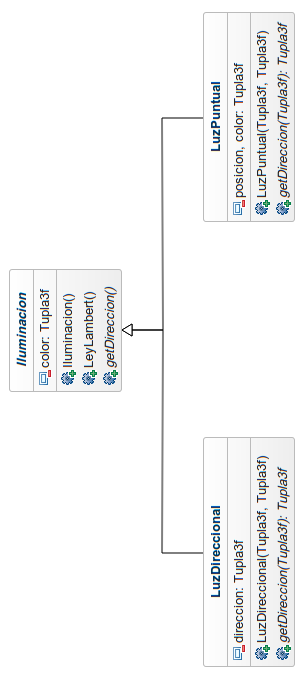
\includegraphics[width=0.6\textwidth]{imagenes/diagrama-clases-iluminacion.png}
	\end{center}
	\caption{Diagrama de clases. Herencia clase abstracta "Iluminacion".}
	\label{fig:etiq_31}
\end{figure}

\begin{figure}[h]
	\begin{center}
		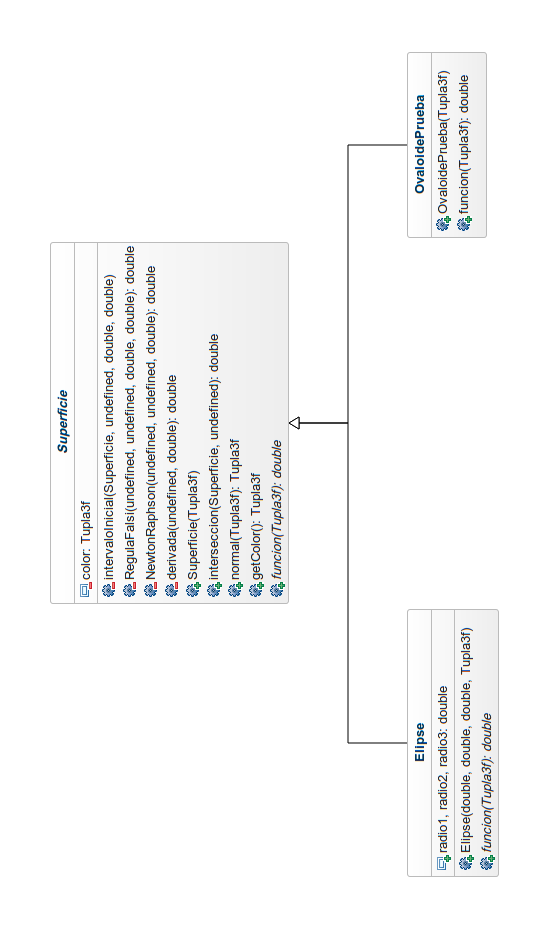
\includegraphics[width=1.0\textwidth]{imagenes/diagrama-clases-superficie.png}
	\end{center}
	\caption{Diagrama de clases. Herencia clase abstracta "Superficie".}
	\label{fig:etiq_32}
\end{figure}

\begin{figure}[h]
	\begin{center}
		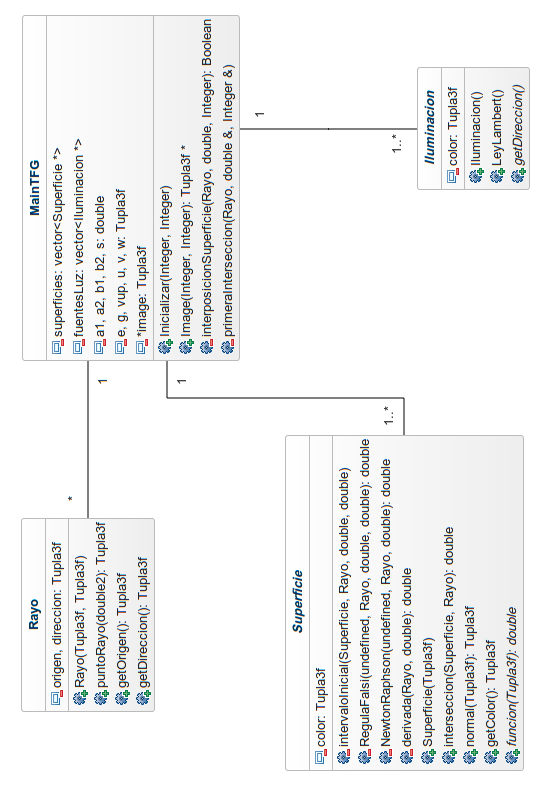
\includegraphics[width=1.0\textwidth]{imagenes/diagrama-clases-completo.png}
	\end{center}
	\caption{Diagrama de clases.}
	\label{fig:etiq_33}
\end{figure}

\chapter{Apéndice B. Instalación.}

Para la instalación del software solo es necesario ir a la carpeta donde se encuentra el archivo $makefile$ desde el terminal y ejecutar la instrucción make en dicho terminal.
${ }$\\

La ejecución del programa solo mostrará la imagen del último ovaloide que visualicé.
${ }$\\

\begin{figure}[h]
	\begin{center}
		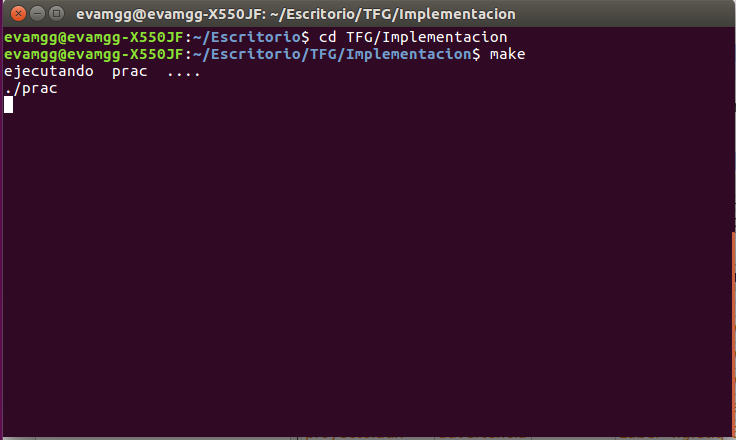
\includegraphics[width=1.0\textwidth]{imagenes/instalacion.png}
	\end{center}
	\caption{Instalación.}
	\label{fig:etiq_41}
\end{figure}

\chapter*{Conclusiones y vías futuras}


%%\nocite{*}
%\bibliography{bibliografia/bibliografia}\addcontentsline{toc}{chapter}{Bibliografía}
%\bibliographystyle{miunsrturl}
%
%\appendix
%\input{apendices/manual_usuario/manual_usuario}
%%\input{apendices/paper/paper}
%\input{glosario/entradas_glosario}
% \addcontentsline{toc}{chapter}{Glosario}
% \printglossary




\thispagestyle{empty}

\nocite{*}
\printbibliography

%\begin{thebibliography}{9}
%	\bibitem{MonRos} S. Montiel-A. Ros, \textit{ Curves and Surfaces }, Graduate Studies in Mathematics v. 69., 2005.
%	
%	\bibitem{Shirley} Peter Shirley, \textit{ Realistic Ray Tracing }, A K Peters/CRC Press, 1874.
	
%	\bibitem{Blinn} James F. Blinn, \textit{A Generalization of Algebraic Surface Drawing}, Jet Propulsion Laboratory, 1982.
	
%	\bibitem{Atkinson} K. Atkinson, \textit{An Introduction to Numerical Analysis}, Wiley,1989.
	
%	\bibitem{Press} W. H. Press and company, \textit{Numerical Recipes in C++: The Art of Scientific Computing}, Cambridge University Press, 2002.

%\end{thebibliography}

\end{document}
